\documentclass[pdflatex,sn-basic]{sn-jnl}
\usepackage[T1]{fontenc}
\usepackage{lmodern}
\usepackage{amsmath}
\usepackage{graphicx}
\usepackage{xcolor}
\usepackage{colortbl}
\usepackage{booktabs}
\usepackage{tabularx}
\usepackage{multirow}
\usepackage{enumitem}
\usepackage{xspace}
\usepackage{etoolbox}
\usepackage{microtype}
\usepackage{placeins}
\let\orcidlogo\relax
\usepackage{orcidlink}

\DeclareRobustCommand{\circled}[1]{\textcircled{\scriptsize #1}}
\setlength{\emergencystretch}{1em}
\newcommand{\system}{\textsc{C2Trace}\xspace}
\newcommand{\NA}{\textsc{n/a}}
\raggedbottom

\renewcommand{\topfraction}{0.95}
\renewcommand{\bottomfraction}{0.9}
\renewcommand{\textfraction}{0.05}
\renewcommand{\floatpagefraction}{0.6}

\def\sectionautorefname{\S}
\def\subsectionautorefname{\S}
\def\subsubsectionautorefname{\S}
\def\figureautorefname{Figure}
\def\tableautorefname{Table}
\def\equationautorefname{Equation}
\def\algorithmautorefname{Algorithm}
\hypersetup{
    colorlinks=true,
    linkcolor=purple,
    anchorcolor=purple,
    citecolor=purple,
    filecolor=purple,
    urlcolor=purple,
    pdftitle={C2Trace: Evidence-Grounded Investigation and Verified Response to Command-and-Control Alerts},
    pdfauthor={Anonymous Author(s)}
}

\newcommand{\RqTracePMacro}{0.873}
\newcommand{\RqTracePMicro}{0.833}
\newcommand{\RqTraceRMacro}{0.719}
\newcommand{\RqTraceRMicro}{0.714}
\newcommand{\RqTraceFMacro}{0.779}
\newcommand{\RqTraceFMicro}{0.769}
\newcommand{\RqTraceTP}{25}
\newcommand{\RqTraceFP}{5}
\newcommand{\RqTraceFN}{10}
\newcommand{\RqResponsePMacro}{1.000}
\newcommand{\RqResponsePMicro}{1.000}
\newcommand{\RqResponseRMacro}{1.000}
\newcommand{\RqResponseRMicro}{1.000}
\newcommand{\RqResponseFMacro}{1.000}
\newcommand{\RqResponseFMicro}{1.000}
\newcommand{\RqResponseTP}{17}
\newcommand{\RqResponseFP}{0}
\newcommand{\RqResponseFN}{0}
\newcommand{\RqMeanLlm}{5.25}
\newcommand{\RqMeanTools}{20.75}
\newcommand{\RqMeanTokens}{83427.9}
\newcommand{\DirectTracePMacro}{0.842}
\newcommand{\DirectTracePMicro}{0.821}
\newcommand{\DirectTraceRMacro}{0.663}
\newcommand{\DirectTraceRMicro}{0.657}
\newcommand{\DirectTraceFMacro}{0.740}
\newcommand{\DirectTraceFMicro}{0.730}
\newcommand{\DirectTraceTP}{23}
\newcommand{\DirectTraceFP}{5}
\newcommand{\DirectTraceFN}{12}
\newcommand{\DirectResponsePMacro}{0.448}
\newcommand{\DirectResponsePMicro}{0.421}
\newcommand{\DirectResponseRMacro}{0.479}
\newcommand{\DirectResponseRMicro}{0.471}
\newcommand{\DirectResponseFMacro}{0.458}
\newcommand{\DirectResponseFMicro}{0.444}
\newcommand{\DirectResponseTP}{8}
\newcommand{\DirectResponseFP}{11}
\newcommand{\DirectResponseFN}{9}
\newcommand{\DirectMeanLlm}{1.00}
\newcommand{\DirectMeanTools}{0.00}
\newcommand{\DirectMeanTokens}{3213.8}
\newcommand{\RqMeanEtime}{120.3}
\newcommand{\DirectTotalTokens}{25710}
\newcommand{\BasCTracePMacro}{0.938}
\newcommand{\BasCTracePMicro}{0.931}
\newcommand{\BasCTraceRMacro}{0.760}
\newcommand{\BasCTraceRMicro}{0.771}
\newcommand{\BasCTraceFMacro}{0.834}
\newcommand{\BasCTraceFMicro}{0.844}
\newcommand{\BasCTraceTP}{81}
\newcommand{\BasCTraceFP}{6}
\newcommand{\BasCTraceFN}{24}
\newcommand{\BasCResponsePMacro}{1.000}
\newcommand{\BasCResponsePMicro}{1.000}
\newcommand{\BasCResponseRMacro}{1.000}
\newcommand{\BasCResponseRMicro}{1.000}
\newcommand{\BasCResponseFMacro}{1.000}
\newcommand{\BasCResponseFMicro}{1.000}
\newcommand{\BasCResponseTP}{51}
\newcommand{\BasCResponseFP}{0}
\newcommand{\BasCResponseFN}{0}
\newcommand{\BasCMeanLlm}{5.25}
\newcommand{\BasCMeanTools}{20.75}
\newcommand{\BasCMeanTokens}{86912.3}
\newcommand{\BasCMeanEtime}{159.4}
\newcommand{\BasCPass}{24}
\newcommand{\BasCFail}{0}
\newcommand{\BasCWrong}{0}
\newcommand{\BasRTracePMacro}{0.698}
\newcommand{\BasRTracePMicro}{0.591}
\newcommand{\BasRTraceRMacro}{0.655}
\newcommand{\BasRTraceRMicro}{0.648}
\newcommand{\BasRTraceFMacro}{0.658}
\newcommand{\BasRTraceFMicro}{0.618}
\newcommand{\BasRTraceTP}{68}
\newcommand{\BasRTraceFP}{47}
\newcommand{\BasRTraceFN}{37}
\newcommand{\BasRResponsePMacro}{1.000}
\newcommand{\BasRResponsePMicro}{1.000}
\newcommand{\BasRResponseRMacro}{0.812}
\newcommand{\BasRResponseRMicro}{0.824}
\newcommand{\BasRResponseFMacro}{0.961}
\newcommand{\BasRResponseFMicro}{0.903}
\newcommand{\BasRResponseTP}{42}
\newcommand{\BasRResponseFP}{0}
\newcommand{\BasRResponseFN}{9}
\newcommand{\BasRMeanLlm}{12.38}
\newcommand{\BasRMeanTools}{27.58}
\newcommand{\BasRMeanTokens}{204406.3}
\newcommand{\BasRMeanEtime}{142.5}
\newcommand{\BasRPass}{12}
\newcommand{\BasRFail}{12}
\newcommand{\BasRWrong}{0}
\newcommand{\PairedTraceCtraceHigher}{13}
\newcommand{\PairedTraceTied}{11}
\newcommand{\PairedTraceReactHigher}{0}
\newcommand{\PairedTraceUndefined}{0}
\newcommand{\PairedTraceComparable}{24}
\newcommand{\PairedTraceN}{24}
\newcommand{\PairedResponseCtraceHigher}{3}
\newcommand{\PairedResponseTied}{18}
\newcommand{\PairedResponseReactHigher}{0}
\newcommand{\PairedResponseUndefined}{3}
\newcommand{\PairedResponseComparable}{21}
\newcommand{\PairedResponseN}{24}
\newcommand{\AoneTracePMicro}{0.767}
\newcommand{\AoneTraceRMicro}{0.657}
\newcommand{\AoneTraceFMicro}{0.708}
\newcommand{\AoneTraceTP}{23}
\newcommand{\AoneTraceFP}{7}
\newcommand{\AoneTraceFN}{12}
\newcommand{\AoneResponsePMicro}{1.000}
\newcommand{\AoneResponseRMicro}{0.765}
\newcommand{\AoneResponseFMicro}{0.867}
\newcommand{\AoneResponseTP}{13}
\newcommand{\AoneResponseFP}{0}
\newcommand{\AoneResponseFN}{4}
\newcommand{\AtwoTracePMicro}{0.692}
\newcommand{\AtwoTraceRMicro}{0.771}
\newcommand{\AtwoTraceFMicro}{0.730}
\newcommand{\AtwoTraceTP}{27}
\newcommand{\AtwoTraceFP}{12}
\newcommand{\AtwoTraceFN}{8}
\newcommand{\AtwoResponsePMicro}{\NA}
\newcommand{\AtwoResponseRMicro}{0.000}
\newcommand{\AtwoResponseFMicro}{\NA}
\newcommand{\AtwoResponseTP}{0}
\newcommand{\AtwoResponseFP}{0}
\newcommand{\AtwoResponseFN}{17}
\newcommand{\AthreeTracePMicro}{0.759}
\newcommand{\AthreeTraceRMicro}{0.629}
\newcommand{\AthreeTraceFMicro}{0.688}
\newcommand{\AthreeTraceTP}{22}
\newcommand{\AthreeTraceFP}{7}
\newcommand{\AthreeTraceFN}{13}
\newcommand{\AthreeResponsePMicro}{1.000}
\newcommand{\AthreeResponseRMicro}{0.765}
\newcommand{\AthreeResponseFMicro}{0.867}
\newcommand{\AthreeResponseTP}{13}
\newcommand{\AthreeResponseFP}{0}
\newcommand{\AthreeResponseFN}{4}
\newcommand{\AfourTracePMicro}{0.750}
\newcommand{\AfourTraceRMicro}{0.771}
\newcommand{\AfourTraceFMicro}{0.761}
\newcommand{\AfourTraceTP}{27}
\newcommand{\AfourTraceFP}{9}
\newcommand{\AfourTraceFN}{8}
\newcommand{\AfourResponsePMicro}{1.000}
\newcommand{\AfourResponseRMicro}{1.000}
\newcommand{\AfourResponseFMicro}{1.000}
\newcommand{\AfourResponseTP}{17}
\newcommand{\AfourResponseFP}{0}
\newcommand{\AfourResponseFN}{0}
\newcommand{\MissingAblMeta}{12}
\newcommand{\AblModelCalls}{92}
\newcommand{\BasCAttempts}{126}
\newcommand{\BasRAttempts}{297}
\newcommand{\BasCModelConfirmed}{126}
\newcommand{\BasRModelConfirmed}{297}
\newcommand{\BasCModelMissing}{0}
\newcommand{\BasCFailed}{0}
\newcommand{\BasRErrors}{0}
\newcommand{\RqModelMissing}{42}
\newcommand{\RqCtwoTraceF}{0.545}
\newcommand{\RqCsevenTraceF}{0.571}


\begin{document}

\title[\system: Investigation and Verified Response]{\system: Evidence-Grounded Investigation and Verified Response to Command-and-Control Alerts}

\author[1]{\fnm{Jun} \sur{Chen}\,\textsuperscript{\orcidlink{0009-0002-4937-6466}}}
\email{jun\_c@hust.edu.cn}

\author[1]{\fnm{Zikai} \sur{Zhou}\,\textsuperscript{\orcidlink{0009-0000-9905-492X}}}
\email{m202572306@hust.edu.cn}

\author[1]{\fnm{Dongxun} \sur{Su}\,\textsuperscript{\orcidlink{0009-0009-6829-7334}}}
\email{dxsssu0114@hust.edu.cn}

\author[1]{\fnm{Feng} \sur{Dong}\,\textsuperscript{\orcidlink{0000-0001-7091-2169}}}
\email{dongfeng@hust.edu.cn}

\author*[1]{\fnm{Haoyu} \sur{Wang}\,\textsuperscript{\orcidlink{0000-0003-1100-8633}}}
\makeatletter\@corauemailfalse\makeatother
\email{haoyuwang@hust.edu.cn}

\author[2]{\fnm{Jingmei} \sur{Chen}\,\textsuperscript{\orcidlink{xxxx-xxxx-xxxx-xxxx}}}
\email{chenjingmei@nsfocus.com}

\affil[1]{\orgname{Huazhong University of Science and Technology}, \orgaddress{\city{Wuhan}, \country{China}}}

\affil[2]{\orgname{NSFOCUS Technologies Group Co., Ltd.}}

\abstract{Command-and-control (C2) alerts flag suspicious communications but do not identify which host objects can be safely modified, especially when legitimate programs host malicious payloads. Predefined playbooks require contextual adaptation, while autonomous large language model (LLM) agents risk premature actions or incomplete verification.
We present \system, an evidence-grounded Windows investigation and response system with three core elements:
(1) persistent C2 knowledge (C2-KB), providing investigation templates, tool-use guidance, evidence rules, and safety principles;
(2) shared case memory (CaseFile), maintaining the evolving strategy tree, host findings, provenance links, and decisions; and
(3) coordinated investigation and response, in which a deterministic controller orchestrates the Planner, Auditor, and Executor using C2-KB and the CaseFile to develop and supplement investigation strategies, resolve targets through read-only queries, execute evidence-backed actions, and verify their effects through fresh host observations.
Across eight controlled Windows scenarios derived from public emulations, \system achieved pooled trace F1 of 0.844, compared with 0.618 for Public ReAct in 48 live trials forming 24 pairs and 0.730 for Offline Direct LLM. Its executed response action F1 was 1.000, compared with 0.903 for Public ReAct and an action-proposal F1 of 0.444 for Offline Direct LLM using fixed evidence without host execution. In the live comparison, \system achieved a 100\% (24/24) independent host-check pass rate, versus 75\% (18/24) for Public ReAct, while reducing mean token usage by 57.5\%.}

\keywords{command and control, alert investigation, automated incident response, large language model agents}

\maketitle

\section{Introduction}
\label{sec:introduction}

\begin{figure}[htbp]
\centering
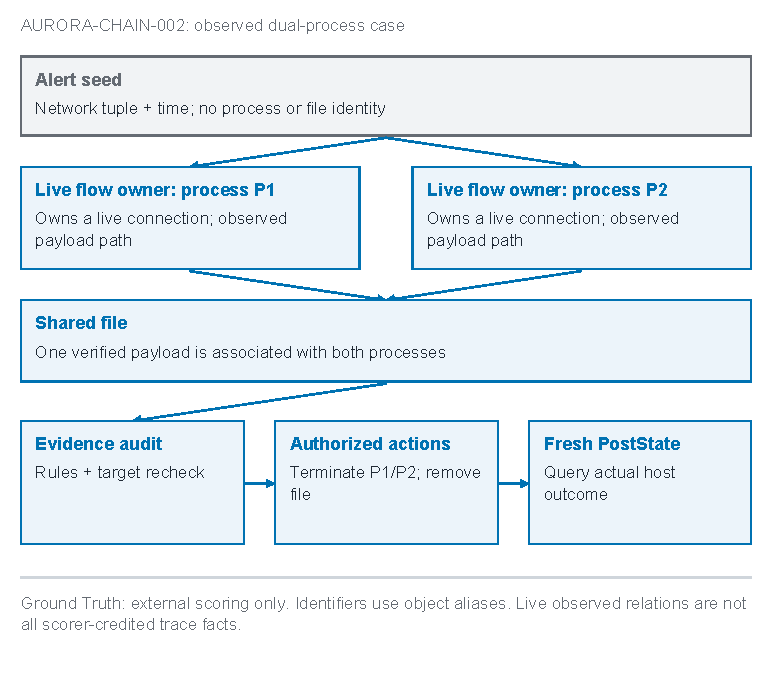
\includegraphics[width=\textwidth]{figures/figure01_motivation.pdf}
\caption{From a C2 alert to distinct process and file response targets. The C2 service on Kali communicates with Windows process P, whose executable is the system file \texttt{rundll32.exe} and whose command line references DLL payload F. Blue labels indicate termination of P and removal of F; the system executable is excluded from deletion. Identifiers are abstracted.}
\label{fig:motivation}
\end{figure}

Command-and-control (C2) communication allows attackers to send instructions to compromised hosts and receive information from them, sustaining remote control that can enable further payload deployment, data theft, and service disruption. Network detectors can flag suspicious C2 communication, but their alerts do not by themselves establish which host process to terminate or which file to remove. This gap complicates response when malicious payloads run through legitimate system programs. \autoref{fig:motivation} illustrates such a case in a controlled Windows scenario derived from the public Wizard Spider emulation plan and Emotet components in the MITRE ATT\&CK Evaluations Library~\citep{ael-wizard-spider-plan}. An Emotet DLL communicates with a C2 service through a process running the legitimate system program \texttt{rundll32.exe}. The required response is to terminate the specific process instance P and remove the DLL payload F while preserving the system executable. Identifying the connection-owning program alone is therefore insufficient: response requires precise attribution from the suspicious connection to the process instance and its associated payload file. These evidence links must distinguish malicious response targets from legitimate host components, and fresh host observations must establish whether the response removed the observed activity.

Existing investigation and response approaches leave three gaps in translating a C2 alert into precise host actions. \textbf{\textit{(Gap 1: Labor-intensive and expertise-dependent investigation)}} Manual investigation requires analysts to query heterogeneous data sources, correlate observations, and document findings, making it labor-intensive~\citep{bridges2023}. The choice and interpretation of evidence also depend on analysts' tacit knowledge, with field studies finding substantial variation in investigation processes and incomplete consideration of relevant evidence~\citep{kersten2023structure,kersten2025field}. \textbf{\textit{(Gap 2: Limited adaptability of predefined playbooks)}} Playbook-based automation standardizes recurring procedures~\citep{cacao2023}, but its flexibility depends on the scenarios, conditions, and actions encoded in advance. Empirical evaluations identify insufficient procedural detail, particularly for junior operators, while research on operations-informed playbooks highlights the need to incorporate organizational dependencies and the operational impact of response~\citep{stevens2022ready,shaked2023operations}. These gaps require contextual adaptation rather than direct reuse of a generic procedure. Moreover, a study of commercial SOAR tools found that greater investigation efficiency could coexist with reduced ticket accuracy and completeness, showing that automation alone does not ensure investigation quality~\citep{bridges2023}. \textbf{\textit{(Gap 3: Insufficient grounding and control of AI-generated actions)}} AI-assisted approaches provide incident-context retrieval, triage and containment recommendations, and investigation summaries~\citep{guided-response2025,kramer2025}. However, evaluations of LLM-based incident analysis report factual inaccuracies and omitted findings, while post-compromise benchmarks reveal incomplete remediation plans and missing verification steps~\citep{kramer2025,secrespond2026}. Moving from advice to autonomous action introduces further risks: response agents can initiate containment before gathering sufficient evidence~\citep{opensec2026}, and tool-using agents can be redirected by instructions embedded in external content~\citep{agentdojo2024,injecagent2024}. For C2 response, these gaps motivate a workflow that adapts investigation to the observed host, grounds each proposed action in evidence for an exact target, constrains execution authority, and verifies the resulting host state.

To bridge these gaps, we present \system, a system for investigating C2 alerts and responding on Windows hosts. Its \textbf{persistent C2 knowledge} base guides the choice of investigative steps and specifies the evidence needed to justify a response. Its \textbf{shared case memory}, the CaseFile, links proposed actions to findings from the current host and to the tool results that support them. For \textbf{coordinated investigation and response}, the Planner draws on both resources to build an investigation strategy, the Auditor checks each proposed action against the evidence for its target and can request further investigation, and the Executor carries out authorized responses. Subsequent host queries verify the effects on the target and the observed C2 activity.

\noindent\textbf{Technical Challenges.} Turning a network alert into a verified host response raises three technical challenges.
\begin{enumerate}[noitemsep, topsep=1pt, partopsep=1pt, listparindent=\parindent, leftmargin=*, label=\circled{\arabic*}]
  \item \textbf{How can reusable C2 knowledge guide an investigation when the alert does not identify the host targets?} Playbook evaluations have found that procedures can omit details operators need to act~\citep{stevens2022ready}. For C2 investigation, a reusable procedure must specify both what to observe and which later query depends on that observation. Inspecting a process, for instance, requires the PID of the owner of the suspicious connection. The dependency can be specified in advance, but only a query on the current host can supply the PID.
  \item \textbf{How can a shared case record preserve the source of each finding and guide the next query?} A field study found that the evidence analysts gathered varied with the alert and the investigator~\citep{kersten2025field}. In a C2 case, a command line may name a DLL while leaving its presence on disk unresolved. The case record must retain the observation behind the candidate path, identify which query can use it, and keep file removal pending while supporting evidence is missing. A chronological tool log alone does not capture those dependencies.
  \item \textbf{How can the system authorize an action on the intended target and verify its effect on a changing host?} In the \texttt{rundll32.exe} scenario, evidence linking a process to the C2 connection can justify terminating that instance without justifying deletion of the system executable. Even after approval, the process may exit and its PID may be reassigned before the termination call. Execution therefore requires a fresh check of the approved target. A successful termination also leaves open whether the payload remains or C2 communication continues, questions that require observations after the action.
\end{enumerate}

\noindent\textbf{Key Insights.} As shown in \autoref{fig:architecture}, \system combines persistent C2 knowledge that guides planning across cases, shared case memory that tracks the evidence in each investigation, and a workflow for coordinated investigation and response. Within this workflow, a deterministic controller coordinates the Planner, Auditor, and Executor as they turn a network alert into a host response and verify its outcome.
\begin{enumerate}[noitemsep, topsep=1pt, partopsep=1pt, listparindent=\parindent, leftmargin=*, label=\circled{\arabic*}]
  \item \textbf{Persistent C2 Knowledge.} The C2 knowledge base (C2-KB) provides an investigation template that describes dependencies among observations and a tool guide that maps investigative steps to operations. Its evidence rules specify which relationships the investigation must establish to justify each proposed response, and its safety guidance identifies objects that require protection. The Planner combines these resources with the alert, the current case summary, and the live tool catalog to build a strategy tree. The tree records prerequisites and outcome branches, leaving arguments that depend on target identity unresolved until host observations supply their values.
  \item \textbf{Shared Case Memory.} Each run starts with a CaseFile containing the alert. The CaseFile holds the strategy tree, findings, evidence links, and audit decisions. As a query completes, the Executor records its result against the issuing node and links each derived finding to that result. The controller uses the recorded outcome to select the next branch and the findings to resolve arguments for queries whose prerequisites are satisfied. When an audit identifies missing evidence, the CaseFile retains both the pending response and the reason for deferral, so that subsequent findings can inform review of the same action.
  \item \textbf{Coordinated Investigation and Response.} The controller validates the Planner's strategy and schedules the Executor's read-only queries. When a response becomes eligible for review, the Auditor checks the proposed operation and target against the case evidence and protection rules. It can approve the action, reject it, or request further evidence. On such a request, the Planner proposes additional queries that the controller attaches to the pending response as prerequisites for renewed review. Approval gives the Executor a short-lived, single-use authorization bound to the target and tool arguments. The tool service validates the authorization and rechecks the target before modifying the host. Fresh queries then check the affected objects and remaining C2 activity, and the case report records the actions taken and their verified or incomplete outcomes.
\end{enumerate}

\noindent\textbf{Evaluation.} We constructed eight controlled Windows C2 scenarios from public emulation material to study investigation and response from an initial network alert. The scenarios cover executable implants, interpreter-hosted DLL and script payloads, a reverse TCP case involving two processes, and an inbound webshell listener. Each scenario provides a reference set of investigation facts and expected actions on specific host objects. Independent host checks capture the effects of the response before the environment is reset. Using this suite, we evaluated whether \system could recover the relevant facts, act on the intended targets, and pass the independent host checks. In one run per scenario, \system achieved pooled F1 scores of 0.769 for trace facts and 1.000 for response actions, and all eight runs passed the host checks. In a separate comparison across 24 retained pairs of trials, pooled F1 was higher for \system than for Public ReAct on both trace facts (0.844 versus 0.618) and response actions (1.000 versus 0.903). The host checks passed in 24 of 24 trials for \system and 18 of 24 for Public ReAct. Mean recorded token usage was 57.48\% lower for \system, although its mean end-to-end execution time was longer (159.4 versus 142.5 seconds). The second baseline, Offline Direct LLM, achieved pooled trace and action-proposal F1 of 0.730 and 0.444 from fixed evidence without host tools. A separate 96-trial component analysis compared the full system with three removal variants over three repetitions per scenario. Without C2-KB and domain guidance, response F1 fell from 1.000 to 0.111; without command-line payload extraction, it was 0.756, including four transport failures. Removing the Auditor reduced response recall from 1.000 to 0.000.

\noindent\textbf{Contributions.} In summary, our work makes three contributions.
\begin{enumerate}[noitemsep, topsep=1pt, partopsep=1pt, listparindent=\parindent, leftmargin=*, label=\circled{\arabic*}]
  \item \textbf{A system for investigating and responding to C2 alerts.} We present \system, which combines a C2 knowledge base for planning with a shared CaseFile that links findings to observations on the current Windows host. The system uses these links to authorize actions on specific targets, rechecks target identity before execution, and verifies the effects of each response through fresh host observations.
  \item \textbf{Eight Windows C2 test scenarios.} We adapted public emulation material into eight controlled scenarios that vary how C2 activity maps to host objects, including cases involving an interpreter-hosted payload or two processes. For each scenario, we specify the facts to recover and the actions expected on particular objects, and independently check host state before resetting the environment.
  \item \textbf{End-to-end evaluation and paired comparison.} All eight scenarios passed independent host checks in the initial evaluation of \system. In a separate comparison across 24 retained pairs of trials, \system achieved higher pooled F1 than Public ReAct for both trace facts (0.844 versus 0.618) and response actions (1.000 versus 0.903). The corresponding host-check pass rates were 24/24 and 18/24.
\end{enumerate}

\section{Background}
\label{sec:background}

\subsection{C2 Communication and Alert Interpretation}
\label{sec:background-c2}

C2 communication enables an adversary to send instructions to compromised hosts and receive their results, often through application protocols also used by legitimate services~\citep{mitre-c2}. Network detectors identify suspicious communication and produce alerts containing network and rule information. Suricata's EVE JSON records, for example, can include source and destination addresses and ports, protocol, timestamp, flow identifier, and detection signature~\citep{suricata-eve}. These observations provide a starting point for investigation, but do not directly identify the current host objects that a response should modify. On Windows, the process owning a connection may execute a separate DLL or script through a legitimate program. Abuse of \texttt{rundll32.exe} illustrates this distinction between the running process, its executable, and the malicious payload~\citep{mitre-rundll32}. Persistence configurations can introduce further objects that maintain access across interruptions~\citep{mitre-persistence}. Precise response therefore requires connecting network evidence to specific process instances, payload files, and relevant persistence entries, with an appropriate operation for each. This attribution determines what to terminate or remove while preserving legitimate host components.

\subsection{LLM Agents for Alert Investigation and Response}
\label{sec:background-llm}

LLM agents offer a way to organize this investigation by generating tool-use plans, interpreting heterogeneous observations, and selecting follow-up queries~\citep{sirbench2026,secrespond2026}. Existing AI-assisted security systems support incident-context retrieval, containment recommendations, and analyst-facing summaries~\citep{guided-response2025,kramer2025}, while tool interfaces such as the Model Context Protocol (MCP) expose named operations and structured arguments for interaction with external systems~\citep{mcp-tools}. These capabilities create opportunities to adapt investigation to the available evidence. Their use in C2 response also raises difficulties beyond producing a coherent explanation. LLM-based incident analysis can omit relevant facts or introduce inaccuracies, and post-compromise evaluations identify incomplete remediation plans and missing verification steps~\citep{kramer2025,secrespond2026}. When plans lead to host modifications, an unsupported process or file association can become an incorrect termination or deletion. Evaluations in an incident-response simulator also find that agents can initiate containment before gathering sufficient evidence~\citep{opensec2026}. Host observations may also contain attacker-controlled text that attempts to redirect tool use~\citep{greshake2023,agentdojo2024,injecagent2024}. Furthermore, a process may exit and its PID may be reused before a proposed action executes~\citep{windows-process}; file contents at a recorded path may also change. A successful tool receipt does not establish that the associated C2 activity has ceased. Applying LLM agents to this task therefore requires grounding proposed actions in current host evidence, separating planning from execution authority, and checking outcomes through fresh observations. These requirements guide the investigation, audit, and execution mechanisms developed in \autoref{sec:methodology}.

\section{Methodology}
\label{sec:methodology}

\subsection{Overview of \system}
\label{sec:system-overview}

\autoref{fig:architecture} presents \system, organized around three elements: \textbf{persistent C2 knowledge}, \textbf{shared case memory}, and \textbf{coordinated investigation and response}. The persistent knowledge component is a curated C2 knowledge base (C2-KB) that provides investigation procedures, tool-use guidance, evidence requirements, and response-safety principles. Shared case memory is maintained in a CaseFile, initialized for each run and updated with strategies, observations, evidence links, audit decisions, and action outcomes. Coordinated investigation and response combines an LLM Planner, a rule-based Auditor, and a tool-invoking Executor under a deterministic workflow controller. A live MCP catalog describes the available tool interfaces.

Given a C2 network alert and the identity of the Windows host to inspect, the controller initializes a CaseFile with the alert as its first finding. The Planner uses the case summary, C2-KB, and the live MCP tool catalog to build a strategy tree for investigation and response. The controller schedules the tree's read-only queries and uses the resulting CaseFile findings to resolve candidate targets, such as the process that owns a suspicious connection. For each proposed response, the Auditor checks whether those findings support the specific operation on its target and records its decision in the CaseFile. If evidence is missing, the Planner uses the audit feedback to add read-only queries, and the Auditor reassesses the proposal once their findings are available. Upon approval, the Executor submits the authorized call to the MCP service, which rechecks the target before modifying the host. Fresh queries then check the affected object and the remaining C2 activity. At the end of the run, \system saves the CaseFile and produces a report linking the evidence and audit decisions to the actions taken, verification results, and final case status.

\begin{figure}[htbp]
\centering
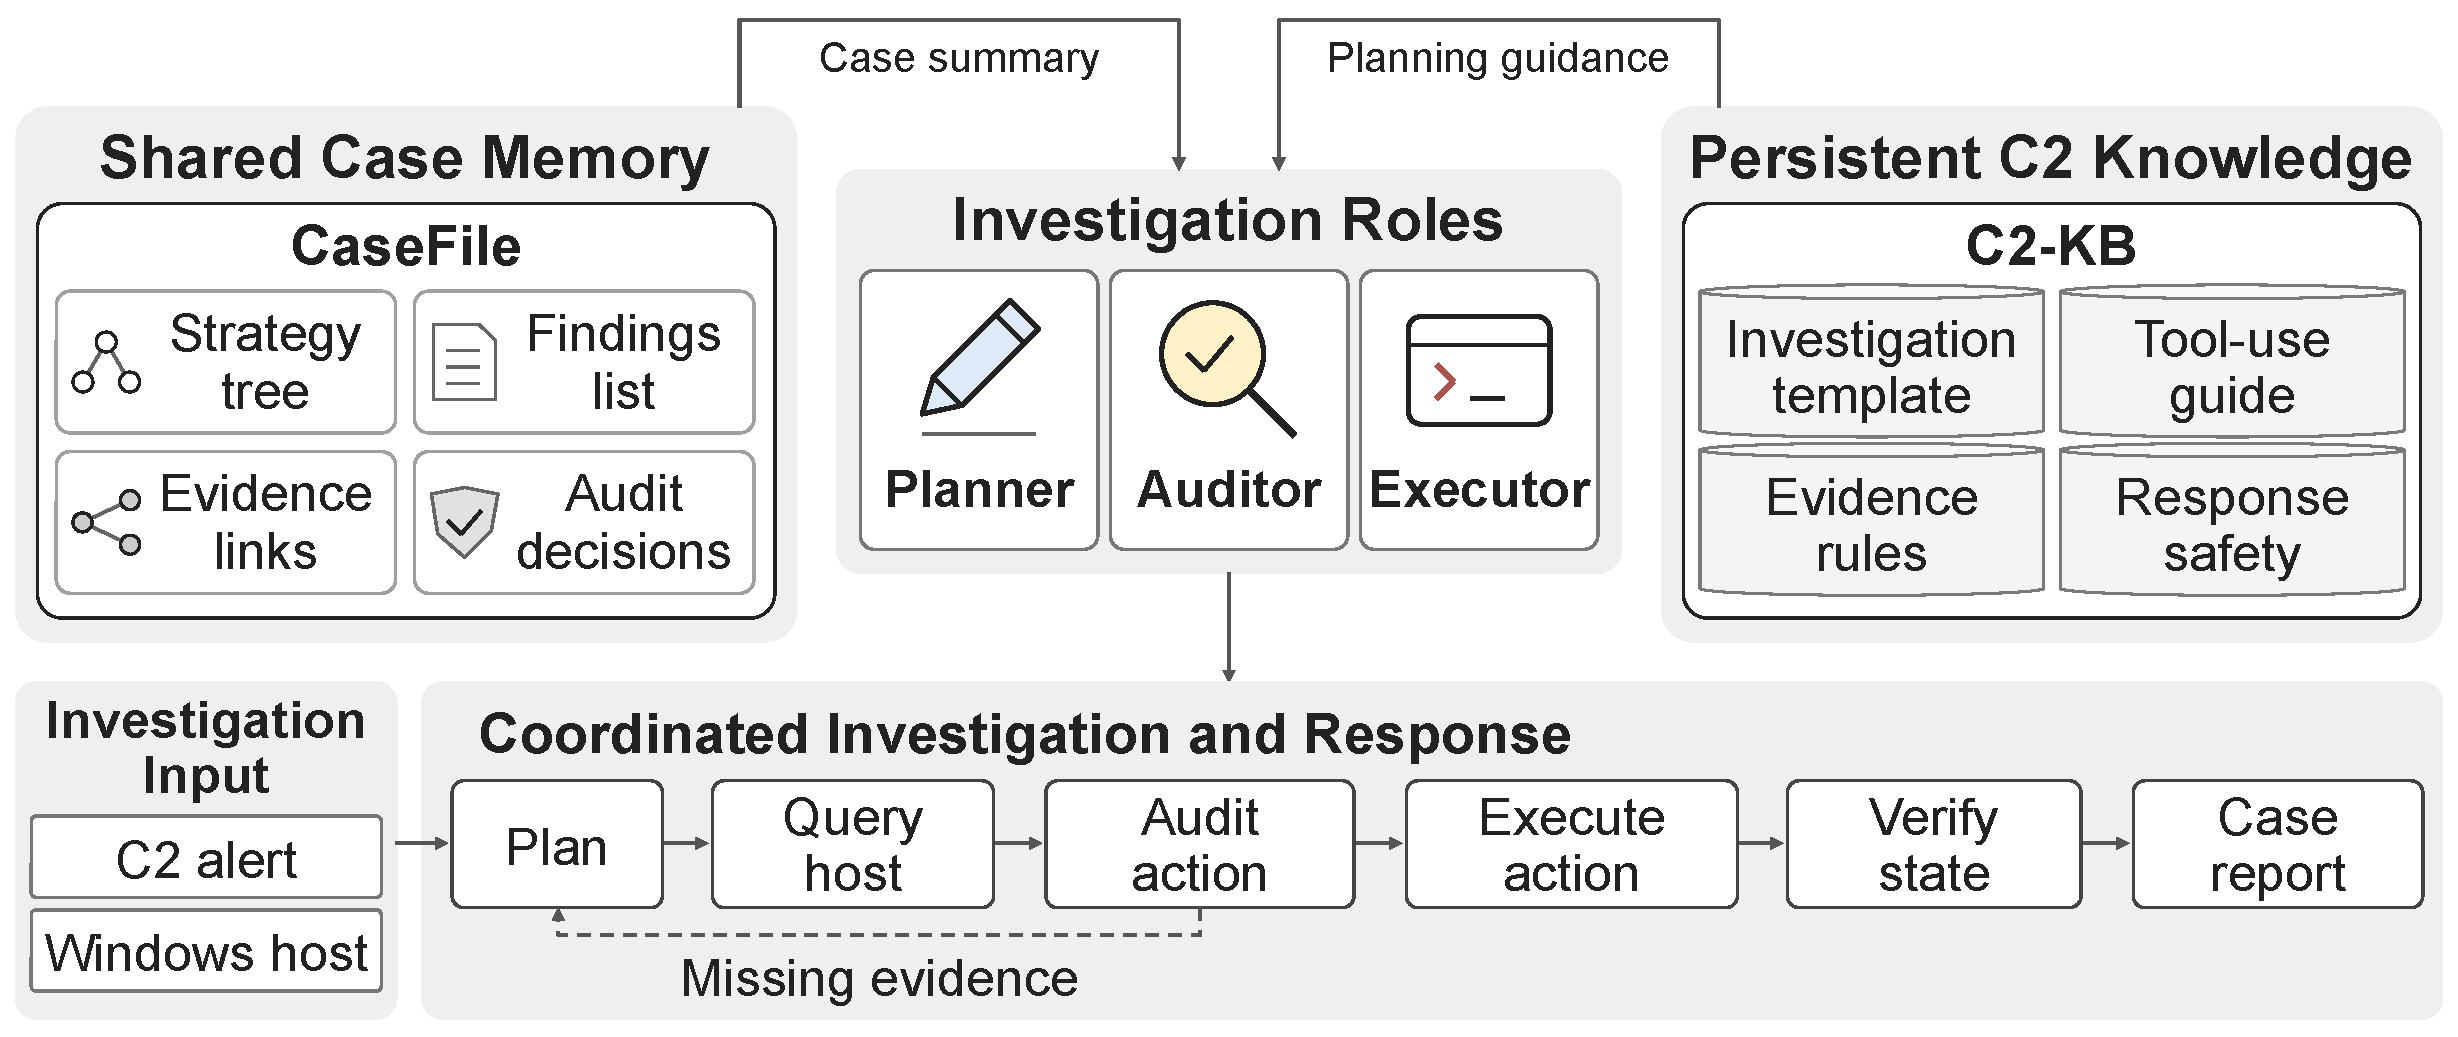
\includegraphics[width=\textwidth]{figures/figure02_architecture.pdf}
\caption{Architecture of \system. C2-KB supplies reusable investigation guidance, while the shared CaseFile maintains strategies, findings, evidence links, and audit decisions. A deterministic controller coordinates the Planner, Auditor, and Executor for investigation and response on the Windows host. These roles use the knowledge and case memory to connect the input C2 alert to evidence-supported host actions and verification results.}
\label{fig:architecture}
\end{figure}

\subsection{Persistent C2 Knowledge}
\label{sec:c2-knowledge}

\system uses C2-KB to provide reusable guidance for investigation and response planning. It contains curated investigation procedures, tool-use guidance, evidence requirements, and response-safety principles. The Planner receives this knowledge as context for initial strategy generation and for additional investigation when auditing identifies missing evidence. C2-KB guides which observations to collect and how to organize subsequent steps, while current host observations establish the identities and state of response targets.

\noindent\textbf{Curated C2 knowledge.} C2-KB organizes general Windows C2 investigation knowledge into four curated text resources, loaded as planning context at runtime. We represent this knowledge pack as
\begin{equation}
\mathcal{K}_{\mathrm{C2}} = (K_{\mathrm{tpl}},K_{\mathrm{tool}},K_{\mathrm{evid}},K_{\mathrm{safe}}),
\label{eq:c2-knowledge}
\end{equation}
where the four components provide complementary guidance:
\begin{itemize}[noitemsep, topsep=1pt, partopsep=1pt, listparindent=\parindent, leftmargin=*]
  \item \textbf{Investigation template ($K_{\mathrm{tpl}}$).} A generic Windows HTTP/HTTPS C2 template describes how to connect a suspicious network endpoint to its owning process, inspect the command line and parent chain, examine file metadata, and query persistence locations and PowerShell history. It also includes post-response checks of network and host-object state.
  \item \textbf{Tool-use guidance ($K_{\mathrm{tool}}$).} A Windows tool guide describes the purposes and typical arguments of read-only investigation and verification tools, together with response tools for process termination, file removal, and persistence cleanup. It provides procedural guidance alongside the live MCP catalog of actual tool interfaces.
  \item \textbf{Evidence requirements ($K_{\mathrm{evid}}$).} Evidence rules describe the links required for different responses: network-to-process attribution for process termination, evidence associating a file with the C2 activity for file removal, and persistence records pointing to the attributed payload for persistence cleanup. Missing links call for further read-only investigation.
  \item \textbf{Response-safety guidance ($K_{\mathrm{safe}}$).} Safety rules require observed target paths and appropriate process identifiers, and reject filename appearance or similarity to another payload as sufficient grounds for removal. These texts guide planning; executable checks in the Auditor and tool service enforce response constraints.
\end{itemize}

\noindent\textbf{Knowledge base construction.} We encode investigation procedures as dependencies between observations. For each stage, $K_{\mathrm{tpl}}$ describes what must already be known and what finding would support the next step. We pair these dependencies with $K_{\mathrm{tool}}$, which identifies the operations that can obtain the required observations and the arguments those operations take. For response planning, $K_{\mathrm{evid}}$ specifies the evidence linking a candidate target to the C2 activity for the proposed action, while $K_{\mathrm{safe}}$ specifies restrictions on which objects that action may affect. These conditions apply across cases. The identity of the target and the evidence supporting an action come from the host under investigation. We maintain the four components as separate text resources and map each to a named field in the knowledge pack.

\noindent\textbf{Runtime knowledge access and planning guidance.} At the start of each run, \system loads the complete $\mathcal{K}_{\mathrm{C2}}$ into the Planner's context. To build the initial strategy, the Planner uses the alert and CaseFile summary to determine which observations are already available, consults the knowledge pack to identify what evidence a proposed response would require, and selects queries from the live MCP catalog to obtain the missing observations. Arguments that depend on future findings remain placeholders in the strategy. If the Auditor later identifies a gap, the Planner receives the pending response, the audit feedback, and an updated CaseFile summary alongside the same knowledge pack. It then proposes additional read-only queries to address that specific gap. Their results become part of the CaseFile that the Auditor inspects when it reviews the response again.

\subsection{Shared Case Memory}
\label{sec:shared-case-memory}

The CaseFile provides shared working memory for each investigation run. It connects the incoming alert to the observations, strategies, decisions, and outcomes produced during investigation and response. Whereas C2-KB supplies reusable procedures, the CaseFile maintains the evolving state of the current case for planning, workflow control, auditing, and reporting.

\noindent\textbf{Case representation and initialization.} Following the four core components shown in \autoref{fig:architecture}, we represent the CaseFile at workflow step $t$ as
\begin{equation}
\mathcal{C}(t) = (C_{\mathrm{tree}}(t), C_{\mathrm{find}}(t), C_{\mathrm{link}}(t), C_{\mathrm{audit}}(t)),
\label{eq:case-representation}
\end{equation}
where the four components are updated as the investigation proceeds.
\begin{enumerate}[noitemsep, topsep=1pt, partopsep=1pt, listparindent=\parindent, leftmargin=*]
  \item \textbf{Strategy tree ($C_{\mathrm{tree}}(t)$).} The Planner represents the strategy as a list of identified nodes linked by prerequisites and outcome branches. Investigation nodes collect observations, decision nodes evaluate conditions, response nodes propose host modifications, and verification nodes check their effects. Prerequisites specify which earlier steps a node depends on, while success and failure branches identify possible successors. A process inspection can thus depend on a network query and leave its PID argument unresolved until the query identifies the owner of the connection. The controller records each node's execution state and selects eligible nodes as results arrive. If the Auditor requests more evidence, the Planner proposes read-only nodes that the controller adds as prerequisites of the pending response, so the same response can be reviewed again after those steps finish.
  \item \textbf{Findings list ($C_{\mathrm{find}}(t)$).} Each entry records a finding with its identifier, type, source, and supporting details. The list starts with the alert and grows as tool results establish facts about the host, such as which process owns the suspicious connection.
  \item \textbf{Evidence links ($C_{\mathrm{link}}(t)$).} Each link connects a tool result to a finding derived from it by recording their identifiers and the relation between them. These links allow a reviewer to trace a finding used in a response decision back to the observation that supports it.
  \item \textbf{Audit decisions ($C_{\mathrm{audit}}(t)$).} Each decision identifies the response node under review and records the Auditor's verdict and rationale. The record names the supporting evidence or the evidence still needed, allowing the controller to advance an approved response, close a rejected branch, or schedule further investigation.
\end{enumerate}

Each run creates a fresh CaseFile from the incoming alert and its source records. Its initial core state is $\mathcal{C}(0)=(\bot,\{f_{\mathrm{alert}}\},\emptyset,\emptyset)$, where $\bot$ denotes an unset strategy and $f_{\mathrm{alert}}$ is the initial alert finding. The CaseFile retains source records, tool results, target-identity records, and a timeline alongside this core state.

\noindent\textbf{Case updates and investigation guidance.} When a read-only query returns, the Executor associates its result with the strategy node, adds any derived findings to $C_{\mathrm{find}}(t)$, and records their links to the result in $C_{\mathrm{link}}(t)$. The controller marks the running node in $C_{\mathrm{tree}}(t)$ as succeeded or failed and follows the corresponding branch. A pending successor on that branch becomes ready once its other prerequisites are satisfied. For example, if a network query identifies the PID that owns a suspicious connection, the process inspection on its success branch can use that PID when it runs. In this way, observations determine which existing nodes run next and supply arguments for their calls. A request for more evidence changes the structure of $C_{\mathrm{tree}}(t)$. The Auditor records the response node and the missing evidence in $C_{\mathrm{audit}}(t)$, and the Planner uses that feedback and the updated case summary to propose read-only investigation nodes. The controller adds the validated nodes to the existing tree and appends their identifiers to the response node's prerequisites, preserving its earlier dependencies. Each new node includes the original response node on its success branch. The controller returns the response node to pending status so that it becomes ready for review only when its dependencies are satisfied. The Auditor then reassesses the same proposed action using the findings recorded during supplementation.

\subsection{Coordinated Investigation and Response}
\label{sec:coordinated-workflow}

\autoref{fig:response-workflow} shows how \system progresses from strategy generation and host investigation to action review, authorized execution, and verification. A deterministic controller validates the Planner's strategy, schedules eligible nodes, and resolves target arguments from host observations. C2-KB guides initial planning and supplementary investigation, while the shared CaseFile carries the strategy, findings, evidence links, and audit decisions across the workflow. The Executor performs read-only queries during investigation; proposals to modify host objects proceed through the Auditor before execution.

\begin{figure}[htbp]
\centering
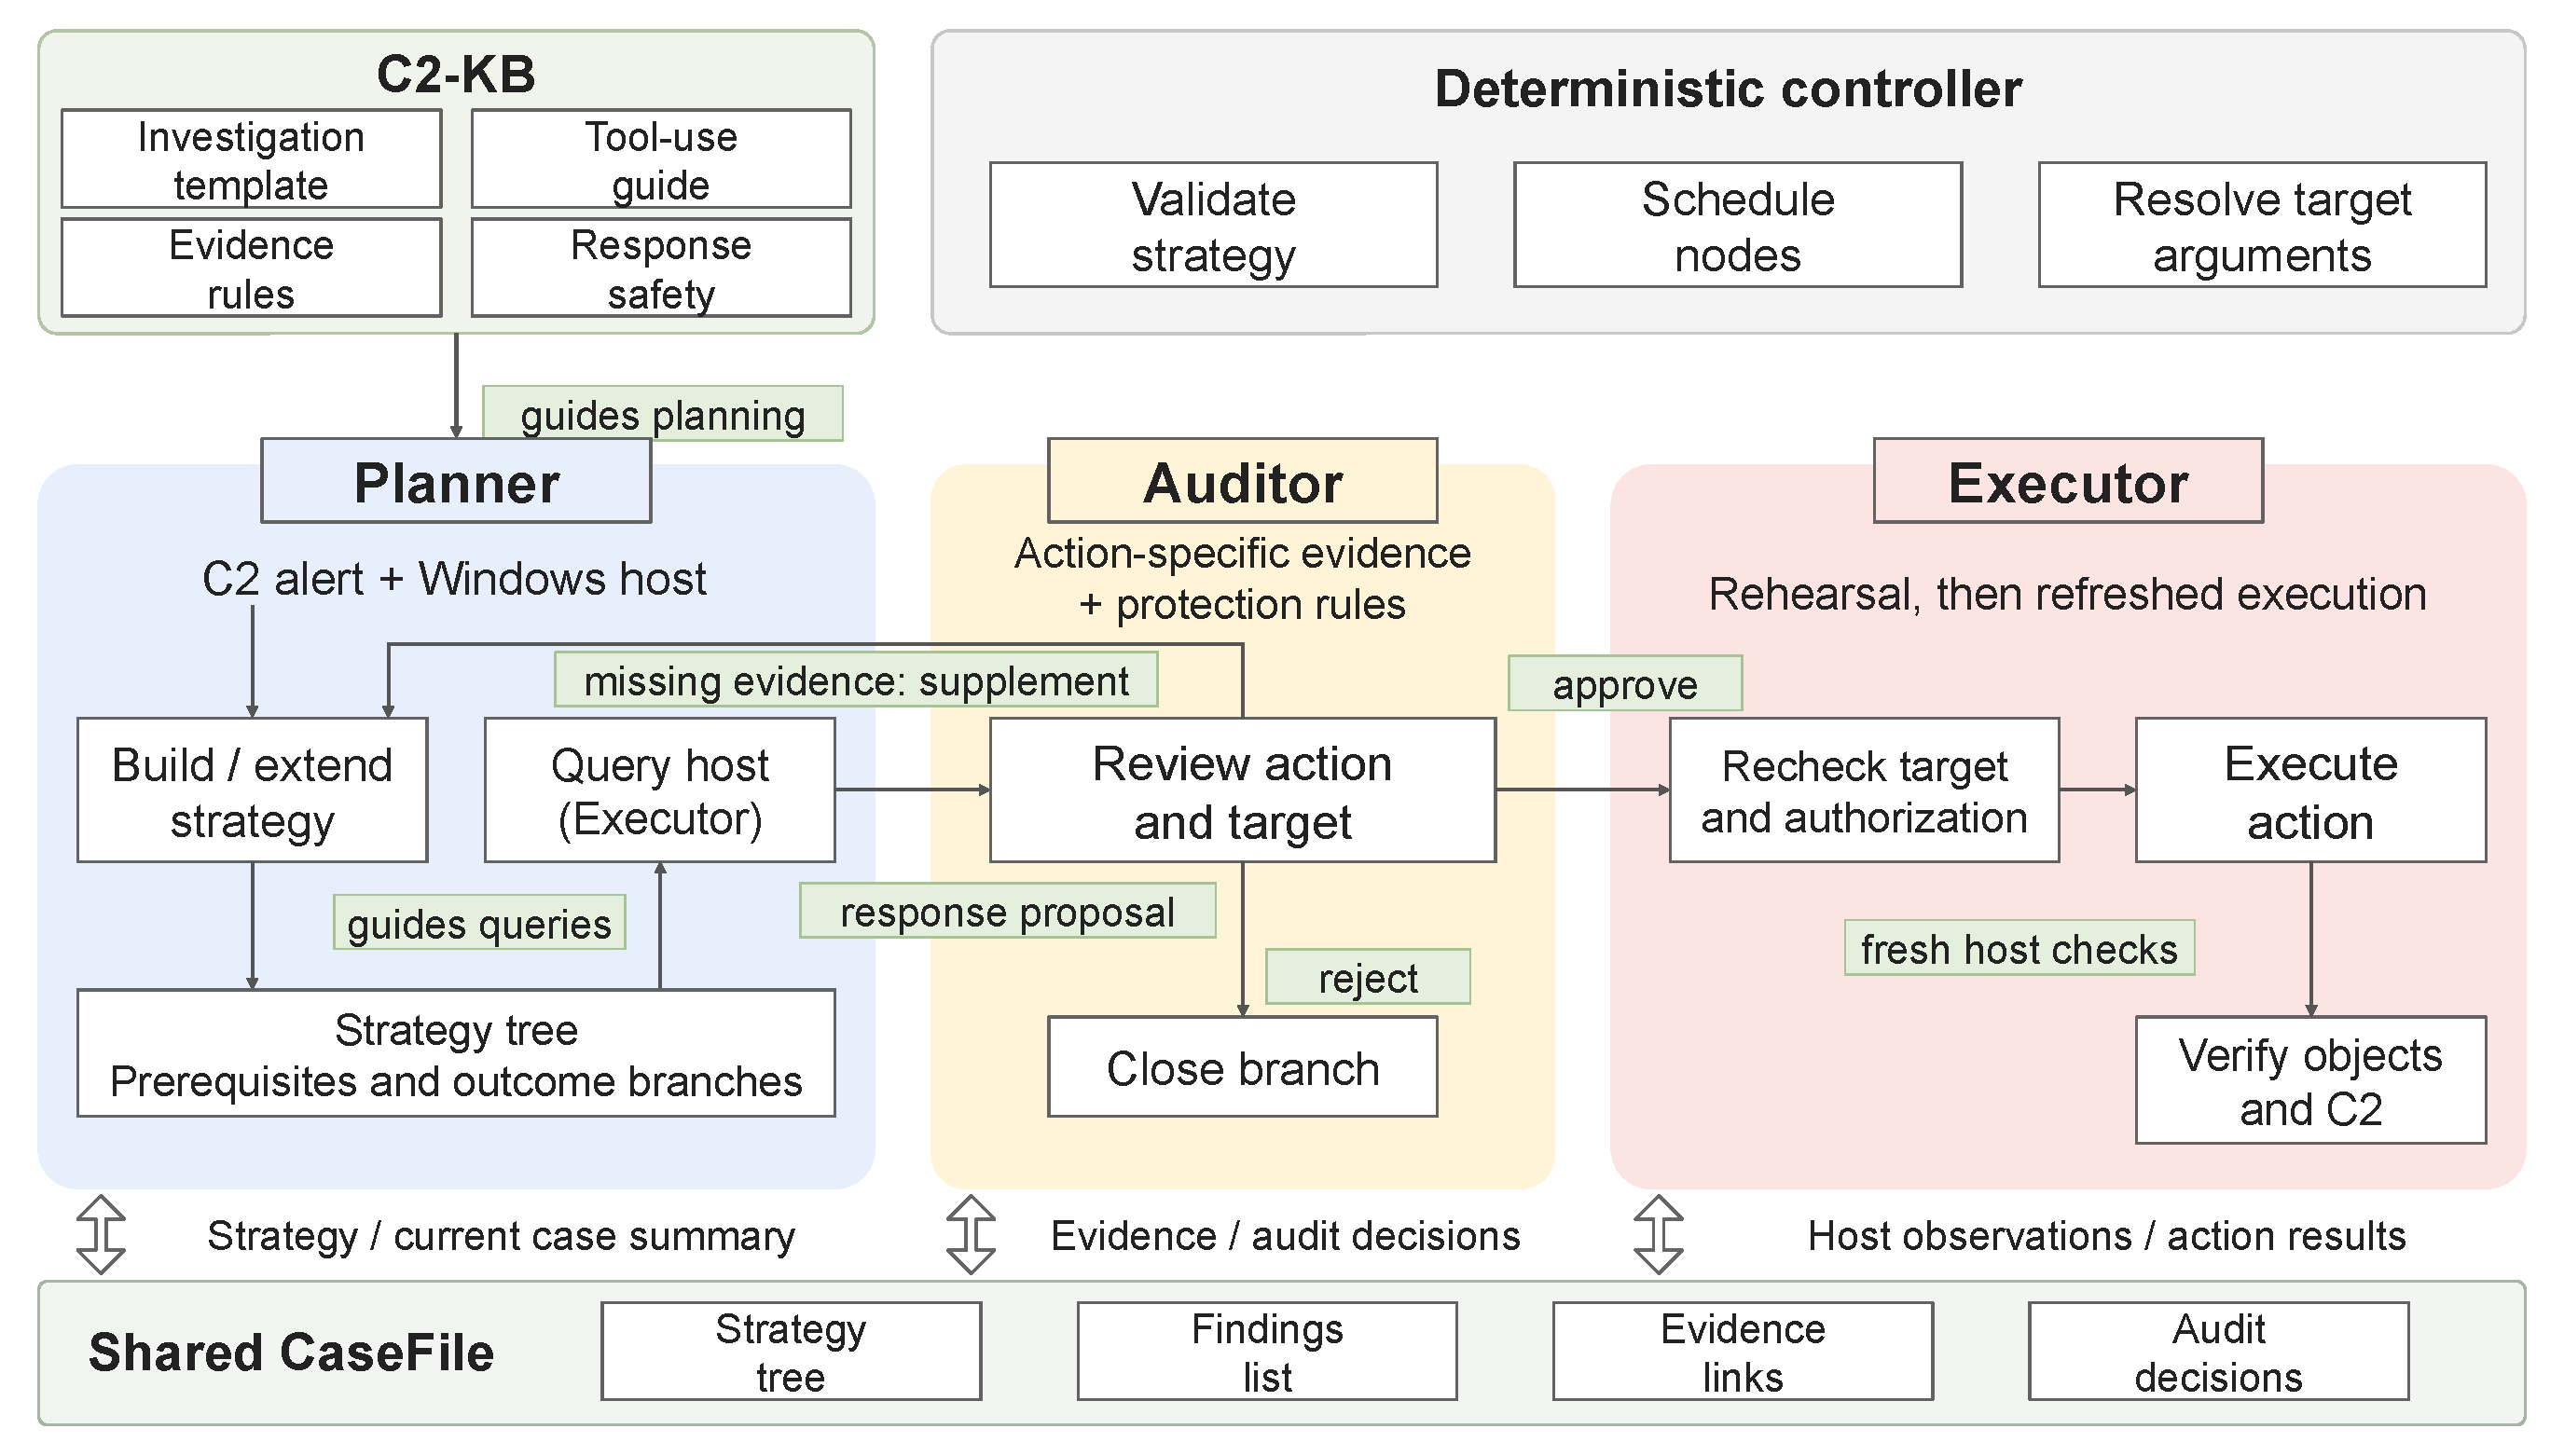
\includegraphics[width=\textwidth]{figures/figure03_response_protocol.pdf}
\caption{Investigation and response workflow of \system. C2-KB guides the Planner in building or extending a strategy tree, whose prerequisites and outcome branches guide host queries. The Auditor reviews concrete response proposals, requests supplementary evidence when needed, and closes rejected branches. Approved actions undergo authorization and target checks before execution, followed by fresh host verification. Hollow bidirectional arrows denote access to and updates of the shared CaseFile.}
\label{fig:response-workflow}
\end{figure}

The Planner first combines the alert, C2-KB, the compact CaseFile summary, and the live MCP tool catalog to generate a structured strategy. Investigation nodes collect observations, decision nodes evaluate conditions, response nodes propose modifications, and verification nodes check outcomes. Each node specifies its objective, tool or condition, arguments, prerequisites, and success or failure branches. Unknown targets remain placeholders to be resolved from host evidence. The generated strategy undergoes structural, dependency, and tool-policy checks, including a requirement that response nodes depend on an evidence-sufficiency decision; selected dependency errors can trigger one constrained repair call. The validated strategy populates $C_{\mathrm{tree}}(t)$ in the CaseFile. The controller then selects ready nodes in sequence and dispatches read-only calls through the Executor, whose results populate $C_{\mathrm{find}}(t)$ and $C_{\mathrm{link}}(t)$. For example, a network observation supplies an owning PID for process inspection, and the resulting command line can expose a payload path for file and persistence queries. The controller resolves identity-sensitive arguments from these observations and advances the corresponding branches. It also supplies a bounded recent-file query as a deterministic investigation supplement. Ordinary tool results advance the existing strategy through these mechanisms rather than triggering a new LLM plan after every call.

The Auditor intervenes when a response node becomes eligible. The Executor prepares a concrete call with resolved arguments, and the Auditor checks whether the current case evidence supports that exact operation and target. Process termination requires an association with the suspicious communication; file removal requires evidence linking the proposed path to the activity; persistence cleanup requires a matching persistence object. Protection checks further constrain the targets. For an interpreter-hosted payload, these distinctions allow the process instance and payload file to be considered separately from the legitimate interpreter executable. The Auditor records approval, rejection, or a request for more evidence in $C_{\mathrm{audit}}(t)$. An LLM-generated explanation can document a rule-supported approval, while deterministic rules determine eligibility. When evidence is missing, the Planner receives the blocked response, audit feedback, updated case summary, and C2-KB to generate additional read-only investigation nodes. The controller attaches these nodes to $C_{\mathrm{tree}}(t)$ and makes the response depend on their completion before renewed review. Rejected proposals close the corresponding response branch. An evidence-sufficiency decision in the strategy therefore enables audit review but does not itself authorize a modification.

The Executor invokes read-only tools during investigation and performs host modifications only through the response controls. Default operation rehearses approved responses without mutation. In the evaluated two-stage protocol, an external controller checks this rehearsal before an execution run reuses the strategy and refreshes observations and audit decisions against the reviewed target. For an approved response, the Auditor issues a signed, short-lived authorization binding the case, prepared call, arguments, and target identity. The MCP service verifies this authorization, performs operation-specific target revalidation, and consumes the one-shot authorization before invoking the modification tool. The Executor records the returned result and its audit association in the CaseFile. After the final response, fresh queries check the affected processes, files, persistence objects, and C2 network state. Completion requires verification findings associated with every executed response and confirmation of the network cleanup state; a successful modification receipt alone is insufficient. Missing verification, failed checks, or remaining artifacts produce distinct incomplete or failure statuses. The controller determines the final status, and the report preserves the investigation evidence, audit decisions, response results, and verification outcomes.

\section{Evaluation}
\label{sec:evaluation}

In this section, we evaluate \system across eight Windows C2 scenarios by measuring the investigation facts it recovers, the actions it takes on host objects, and the host state after response. We compare \system with Public ReAct for live investigation and response and with Offline Direct LLM for fact recovery and action proposals from fixed evidence. A separate component analysis examines three removal variants.

\noindent\textbf{Research Questions.}
We evaluate \system to answer three research questions:
\begin{itemize}[leftmargin=*, itemsep=3pt, topsep=3pt]
  \item \textbf{RQ1 (Effectiveness).} How effective is \system at investigating and responding to C2 alerts?
  \item \textbf{RQ2 (Baseline Comparison).} How does \system compare with the baseline in effectiveness and efficiency?
  \item \textbf{RQ3 (Component Analysis).} How do investigation and response outcomes change when individual components of \system are removed?
\end{itemize}

\noindent\textbf{Test Dataset Construction.} We constructed eight executable Windows C2 scenarios from selected behaviors in public emulation material. As \autoref{tab:scenarios} shows, C1--C2 derive from Aurora demonstrations, C3--C7 from the ATT\&CK Evaluations Library, and C8 from a CTID webshell emulation~\citep{aurora2026,attackevals-ael-repo,ctid-ael-repo}. The cases expose different relationships between a network alert and the objects that a responder must identify. An executable can itself be the payload, a legitimate host program can load a separate DLL or script, and a single case can involve two processes. C8 exercises an inbound listener, extending coverage beyond outbound connections.

For each scenario, we selected the source behavior to reproduce, identified the processes and files involved, and scripted the steps needed to deploy the payload and exercise its C2 channel in a controlled Windows VM. We documented how the scripted steps corresponded to the public source and specified which host and network observations the evaluator would need to identify the deployed targets. During execution, Suricata captured the network event that served as the starting point for the investigation. 

We paired each scenario with a scoring template that specifies the trace facts an investigation should recover and the actions expected on particular host objects. The template defines how to identify each object while leaving runtime values to be supplied by the trial. For instance, a process reference can combine its PID, creation time, and executable path. After execution, the evaluation controller fills the reference from the deployment records, the network event, and host observations captured before response. The investigator starts from the alert and obtains target identities through host queries, while the evaluator uses the completed reference to score the run. The final two columns of \autoref{tab:scenarios} give the per-case counts, totaling 35 trace facts and 17 expected actions across the suite. For the effectiveness and baseline trials, independent host checks before environment recovery establish whether the expected response took effect on the selected targets.

\begingroup
\let\table\tableorg
\let\endtable\endtableorg
\begin{table}[htbp]
\centering
\caption{Overview of the eight Windows C2 test scenarios.}
\label{tab:scenarios}
\small
\renewcommand{\arraystretch}{1.15}
\setlength{\tabcolsep}{3pt}
\resizebox{\linewidth}{!}{%
\begin{tabular}{llllrr}
\toprule
\textbf{Case} & \textbf{Source} & \textbf{C2 channel} & \textbf{Host carrier / payload} & \textbf{Trace facts} & \textbf{Actions} \\
\midrule
\rowcolor{black!6}
C1: Aurora 1 & Aurora & mTLS & EXE & 4 & 2 \\
C2: Aurora 2 & Aurora & Reverse TCP & Two instances / one EXE & 6 & 3 \\
\rowcolor{black!6}
C3: SideTwist & AEL & HTTP/XOR & EXE & 4 & 2 \\
C4: Exaramel & AEL & HTTPS & EXE & 4 & 2 \\
\rowcolor{black!6}
C5: Emotet & AEL & HTTP & rundll32 / DLL & 4 & 2 \\
C6: Carbanak & AEL & HTTPS & cscript / JS & 4 & 2 \\
\rowcolor{black!6}
C7: PlugX & AEL & HTTP/RC4 & python / PY & 4 & 2 \\
C8: WebShell & CTID & Inbound HTTP & EXE listener & 5 & 2 \\
\bottomrule
\end{tabular}
}
\end{table}

\endgroup

\noindent\textbf{Experimental Setup.} All experiments used \texttt{deepseek-v4.1-flash}, including the Public ReAct and Offline Direct LLM comparisons. We ran the live trials in a controlled Windows 10 VM, with Kali hosting scenario services and deployment channels. In \system, the Planner uses the model to generate investigation strategies, and the Auditor can use it to explain decisions made by deterministic rules. RQ2 includes two baselines: Public ReAct investigates and acts on the live host, while Offline Direct LLM produces findings and response proposals without calling host tools. In the live comparison, \system and Public ReAct used the same alert conditions, low-level Windows tools, and scorer, each with its own workflow and call limits. We set the temperature to 0.0 for the Planner and Public ReAct and to 0.1 for the Auditor's optional explanations.

Each live trial began with a Suricata alert and the identity of the host to inspect. The investigator queried the host to identify response targets, and the evaluator scored the results against a separate scenario reference. \system rehearsed its strategy without modifying the host, then collected fresh observations and repeated the audit before executing approved actions. For RQ1, we ran \system once per scenario, yielding eight runs. For the live RQ2 comparison, we ran \system and Public ReAct three times each per scenario, yielding 24 pairs (48 trials) matched by scenario and repetition. In RQ1, the live RQ2 trials, and RQ3, the evaluator independently checked the host after the response and before environment recovery. For the offline RQ2 comparison, we supplied a frozen, de-labelled evidence bundle for each scenario, ran one inference, and scored the reported trace facts and proposed actions against the scenario references. These eight inferences provide proposal scores and token counts, with no executed actions or post-response host measurements. For RQ3, we evaluated the full system and three component-removal variants three times per scenario, yielding 24 trials per configuration and 96 trials in total. Each experiment group uses separate ground-truth references for scoring, and we report its results separately.

% \begin{figure}[htbp]
% \centering
% 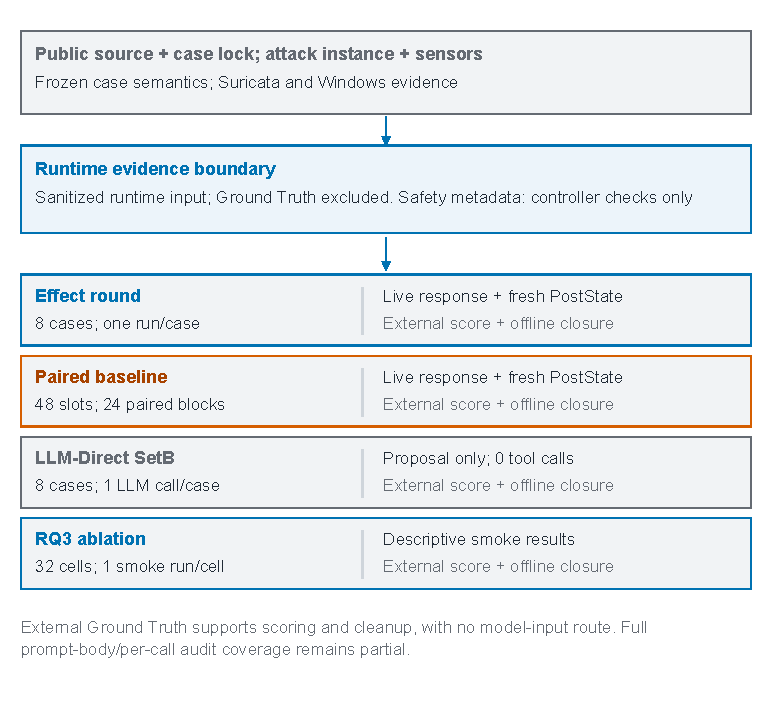
\includegraphics[width=\textwidth]{figures/figure04_evidence_pipeline.pdf}
% \caption{Experimental design with four separately reported populations: eight effectiveness runs, 24 C2Trace--Public ReAct pairs (48 runs), 32 ablation cells, and eight offline LLM-Direct inferences. Each ablation cell is one smoke-mode execution; A1--A4 remove auditing, target binding, prechecks, and internal post-verification, respectively. Effectiveness and paired runs include independent fresh host-state measurement before external cleanup. Ablation evidence remains limited to the available smoke records. LLM-Direct produces trace and action proposals without host-tool execution or measured PostState, so proposal scores are distinct from executed-action scores. Ground Truth supplies external scoring references; resource measures use available run records. Input separation denotes the experimental design, with incomplete prompt and call-level audit coverage for baseline and ablation}
% \label{fig:evidence-pipeline}
% \end{figure}

\noindent\textbf{Evaluation Metrics.} We score investigation and response separately against the reference for each trial. For investigation, a match is a reported trace fact that agrees with a reference fact. For response, both the executed operation and its target object must match the expected action. For each task $d\in\{\mathrm{trace},\mathrm{action}\}$, let $TP_d$ count matches, $FP_d$ unmatched outputs, and $FN_d$ missed reference items. We compute precision, recall, and F1 as
\begin{equation}
P_d=\frac{TP_d}{TP_d+FP_d},\qquad
R_d=\frac{TP_d}{TP_d+FN_d},\qquad
F_{1,d}=\frac{2TP_d}{2TP_d+FP_d+FN_d}.
\end{equation}
We apply the scorer's definedness rule: when the system produces no output for a task, precision and F1 are \NA{}, and recall is zero if reference items exist. When outputs and reference items both exist but none match, F1 is zero. For each task, let $\mathbf{c}_i=(TP_i,FP_i,FN_i)$ pool the counts across retained repetitions of scenario $i$. For any metric $m\in\{P,R,F_1\}$, let $D_m$ contain the scenarios for which $m(\mathbf{c}_i)$ is defined. We report
\begin{equation}
m_{\mathrm{micro}}=m\!\left(\sum_i\mathbf{c}_i\right),\qquad
m_{\mathrm{macro}}=\frac{1}{|D_m|}\sum_{i\in D_m}m(\mathbf{c}_i).
\end{equation}

We measure response completion from independent host observations collected before environment recovery. For each of the $N$ trials with a measured PostState in a given evaluation group, let $h_j=1$ if the required checks pass and $h_j=0$ otherwise. These checks establish whether the selected C2 connection or listener and the targeted host objects are absent as required, and whether protected control processes remain active. We report the pass count $\sum_{j=1}^{N}h_j$ and the pass rate $(\sum_{j=1}^{N}h_j)/N$. For efficiency, we report the mean per trial of each recorded measure: LLM calls, tool calls, tokens, and end-to-end elapsed time in seconds. Elapsed time includes the evaluation controller's orchestration.

% \subsection{Setting and Public-Source Scenarios}

% We analyze archived executions in one controlled Windows VM rather than a production deployment. The eight scenarios in Table~\ref{tab:scenarios} cover executable implants, interpreter-hosted DLL or script payloads, a dual-process reverse-TCP case, and an inbound webshell listener. Their sources include Aurora demonstrations, the ATT\&CK Evaluations Library (AEL), and CTID emulation material~\citep{aurora2026,attackevals-ael-repo,ctid-ael-repo}. They are bounded source-derived slices, not complete campaigns or proof of native malware-family fidelity. In particular, C7 implements a PlugX-like HTTP/RC4 protocol in Python rather than a native PlugX DLL. Protocol labels describe the source implementation; the selected EVE events report TCP transport and do not independently validate every higher-level protocol label. C1 includes an environment-query ability and C2 an ARP-query ability. These exercised behaviors do not imply coverage of other public-source steps.

% Each live evaluation separates experimental orchestration from model attribution. The controller starts a scenario, obtains an independent network alert, protects experiment-control objects, and supplies the permitted runtime evidence. \system uses a dry-run rehearsal and a refreshed execute run; the Public ReAct runner has its own investigation and execution stages. External Ground Truth and scoring projections match recovered trace facts and response objects after the run. Fresh PostState is measured before controller recovery, checking the selected target and protected controls. Infrastructure validity, measured response, wrong-target indicators, trial classification, and cleanup are separate fields. A later successful cleanup cannot change a failed measured response. Figure~\ref{fig:evidence-pipeline} distinguishes the four retained experiment populations; we never pool them into one overall result.

% For C5, we build the public Emotet emulation DLL and companion control service, with laboratory network and build adaptations~\citep{ael-emotet-component}. A dedicated execution script organizes controlled deployment, HTTP C2 interaction, and a process-enumeration task. CALDERA supports agent discovery in the common experimental environment, including identification of the control and driver agents. The DLL deployment and Emotet C2 task use native components and the dedicated execution adapter rather than native CALDERA operations.

% After response and before external cleanup, an independent evaluation procedure reobserves host state. For the illustrated run, the target connection, process, and DLL file were absent, while the control agent remained alive. These observations assess the actual response outcome separately from individual tool-call success. Excluding the system executable from deletion is a response-scope decision; its post-response integrity was not independently measured in this run.


% % Begin figures/figure04_evidence_pipeline.tex
% \begin{figure}[htbp]
% \centering
% 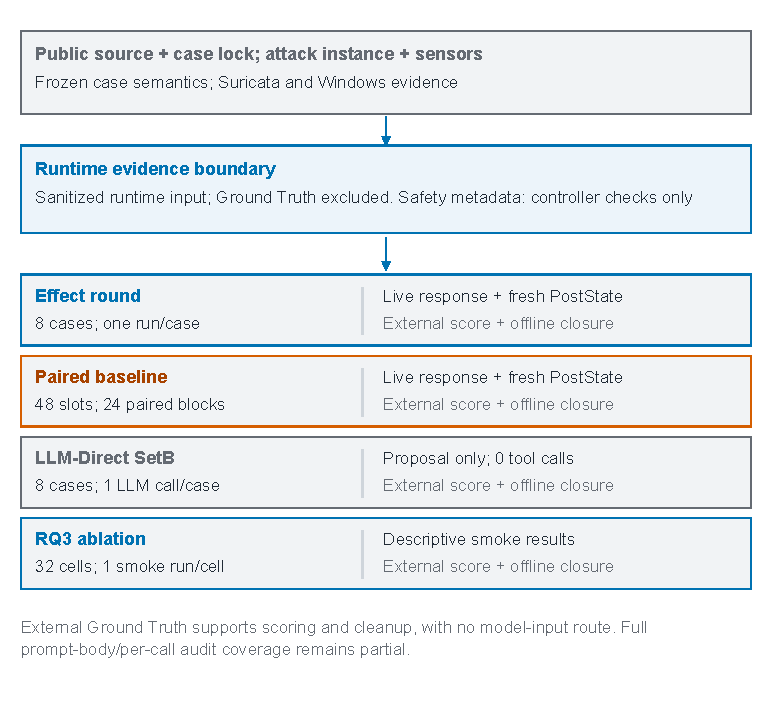
\includegraphics[width=\textwidth]{figures/figure04_evidence_pipeline.pdf}
% \caption{Experimental design with four separately reported populations: eight effectiveness runs, 24 C2Trace--Public ReAct pairs (48 runs), 32 ablation cells, and eight offline LLM-Direct inferences. Each ablation cell is one smoke-mode execution; A1--A4 remove auditing, target binding, prechecks, and internal post-verification, respectively. Effectiveness and paired runs include independent fresh host-state measurement before external cleanup. Ablation evidence remains limited to the available smoke records. LLM-Direct produces trace and action proposals without host-tool execution or measured PostState, so proposal scores are distinct from executed-action scores. Ground Truth supplies external scoring references; resource measures use available run records. Input separation denotes the experimental design, with incomplete prompt and call-level audit coverage for baseline and ablation}
% \label{fig:evidence-pipeline}
% \end{figure}

% % End figures/figure04_evidence_pipeline.tex


% \subsection{Measurements and Aggregation}

% Trace scoring matches case-specific facts about the observed source activity and attributed host objects. Response action scoring matches the required object-specific actions; its precision and recall do not replace fresh PostState. We recompute precision and recall from archived $TP$, $FP$, and $FN$, retaining the scorer's denominator semantics. When precision is undefined because no prediction exists, precision and F1 remain \NA{} even if recall is zero. When predictions exist but none match and both relevant denominators are nonzero, F1 is zero. We do not replace either situation with the other.

% For repeated cases, we pool counts within each case before computing that case's metric. The case macro is the mean of available case metrics, with the non-null count $n/N$ stated when necessary. Pooled micro combines counts over all retained trials before computing the metric. This distinction matters when a system makes no response prediction in an entire case: a macro F1 over seven defined cases is not an eight-case success rate. We report all retained trials, including evaluation failures and wrong-target outcomes. Recorded costs include LLM calls, tool calls, and returned token usage. Controller end-to-end duration includes orchestration around the case; it is distinct from case, investigation, response, and verification durations. Costs are not inferred API invoices.

% All numerical tables are generated from a locally verified result file whose companion maps each displayed entry to source SHA-256, JSON fields, and derivation. The offline reconstruction checks archived originals against independent scoring and closure outputs without rerunning the scorer or executing scenarios. Our analysis is descriptive: we report no confidence intervals, significance tests, or causal estimates.


\subsection{RQ1 (Effectiveness)}

We evaluated \system once on each of the eight Windows C2 scenarios, starting from a network alert and scoring the recovered facts and executed actions against the scenario reference. After response, an independent procedure checked the host before environment recovery. Each run averaged 120.3 seconds, 5.25 LLM calls, 20.75 tool calls, and 83,427.9 tokens. \autoref{tab:effectiveness} presents the investigation accuracy, response accuracy, and host-check outcome for each scenario.

\begingroup
\let\table\tableorg
\let\endtable\endtableorg
\begin{table}[htbp]
\centering
\caption{Effectiveness of C2Trace across eight Windows C2 scenarios, with one trial per scenario.}
\label{tab:effectiveness}
\small
\renewcommand{\arraystretch}{1.15}
\setlength{\tabcolsep}{6pt}
\begin{tabular}{lrrc}
\toprule
\textbf{Case} & \textbf{Trace F1} & \textbf{Response F1} & \textbf{Fresh PostState} \\
\midrule
\rowcolor{black!6}
C1: Aurora 1 & 0.857 & 1.000 & Pass \\
C2: Aurora 2 & 0.545 & 1.000 & Pass \\
\rowcolor{black!6}
C3: SideTwist & 0.857 & 1.000 & Pass \\
C4: Exaramel & 0.857 & 1.000 & Pass \\
\rowcolor{black!6}
C5: Emotet & 0.857 & 1.000 & Pass \\
C6: Carbanak & 0.857 & 1.000 & Pass \\
\rowcolor{black!6}
C7: PlugX & 0.571 & 1.000 & Pass \\
C8: WebShell & 0.833 & 1.000 & Pass \\
\midrule
Macro & 0.779 & 1.000 & -- \\
Micro & 0.769 & 1.000 & -- \\
\bottomrule
\end{tabular}
\end{table}
\endgroup

\noindent\textbf{Trace coverage.} Across the eight runs, \system recovered 25 of 35 reference facts, missed 10, and reported 5 additional observations that did not match the reference. Pooled precision was 0.833 and recall was 0.714, yielding a micro F1 of 0.769. The macro F1 was 0.779. The lower recall indicates that missing reference facts accounted for more errors than additional unmatched observations. Performance varied across scenarios. Five cases achieved trace F1 of 0.857, while the two-process case (C2) and the PlugX-like emulation (C7) had the lowest scores, 0.545 and 0.571, respectively. These results show that investigation coverage remained incomplete across the suite, with the largest gaps in C2 and C7.

\noindent\textbf{Verified response.} \system executed all 17 expected actions on their intended targets, yielding precision, recall, and F1 of 1.000 for response actions. Independent host checks passed in all eight runs. The targeted connections or listeners and the host objects designated for removal were absent as required, while protected control processes remained active. The agreement between action matching and host observations supports response completion for the targets specified in these scenarios. In particular, C2 and C7 both achieved response F1 of 1.000 and passed the host checks despite their lower trace scores. In those runs, the investigation recovered enough information to select the required response objects while leaving some reference facts unresolved.

\subsection{RQ2 (Baseline Comparison)}

We compared \system with Public ReAct across eight scenarios, with three repetitions per system and scenario. The 48 retained trials form 24 pairs matched by scenario and repetition. Both systems used \texttt{deepseek-v4.1-flash}, the same alert conditions, low-level Windows tools, and scorer, with their respective workflows and call limits. Setup failures and model-service failures before a valid model response were replaced within the same trial slot, while failures following normal model output remained in the comparison. \autoref{tab:baseline} summarizes accuracy and resource usage, and \autoref{fig:rq2-comparison} compares aggregate F1, scenario-level trace F1, and mean resource usage.

\begin{figure}[htbp]
\centering
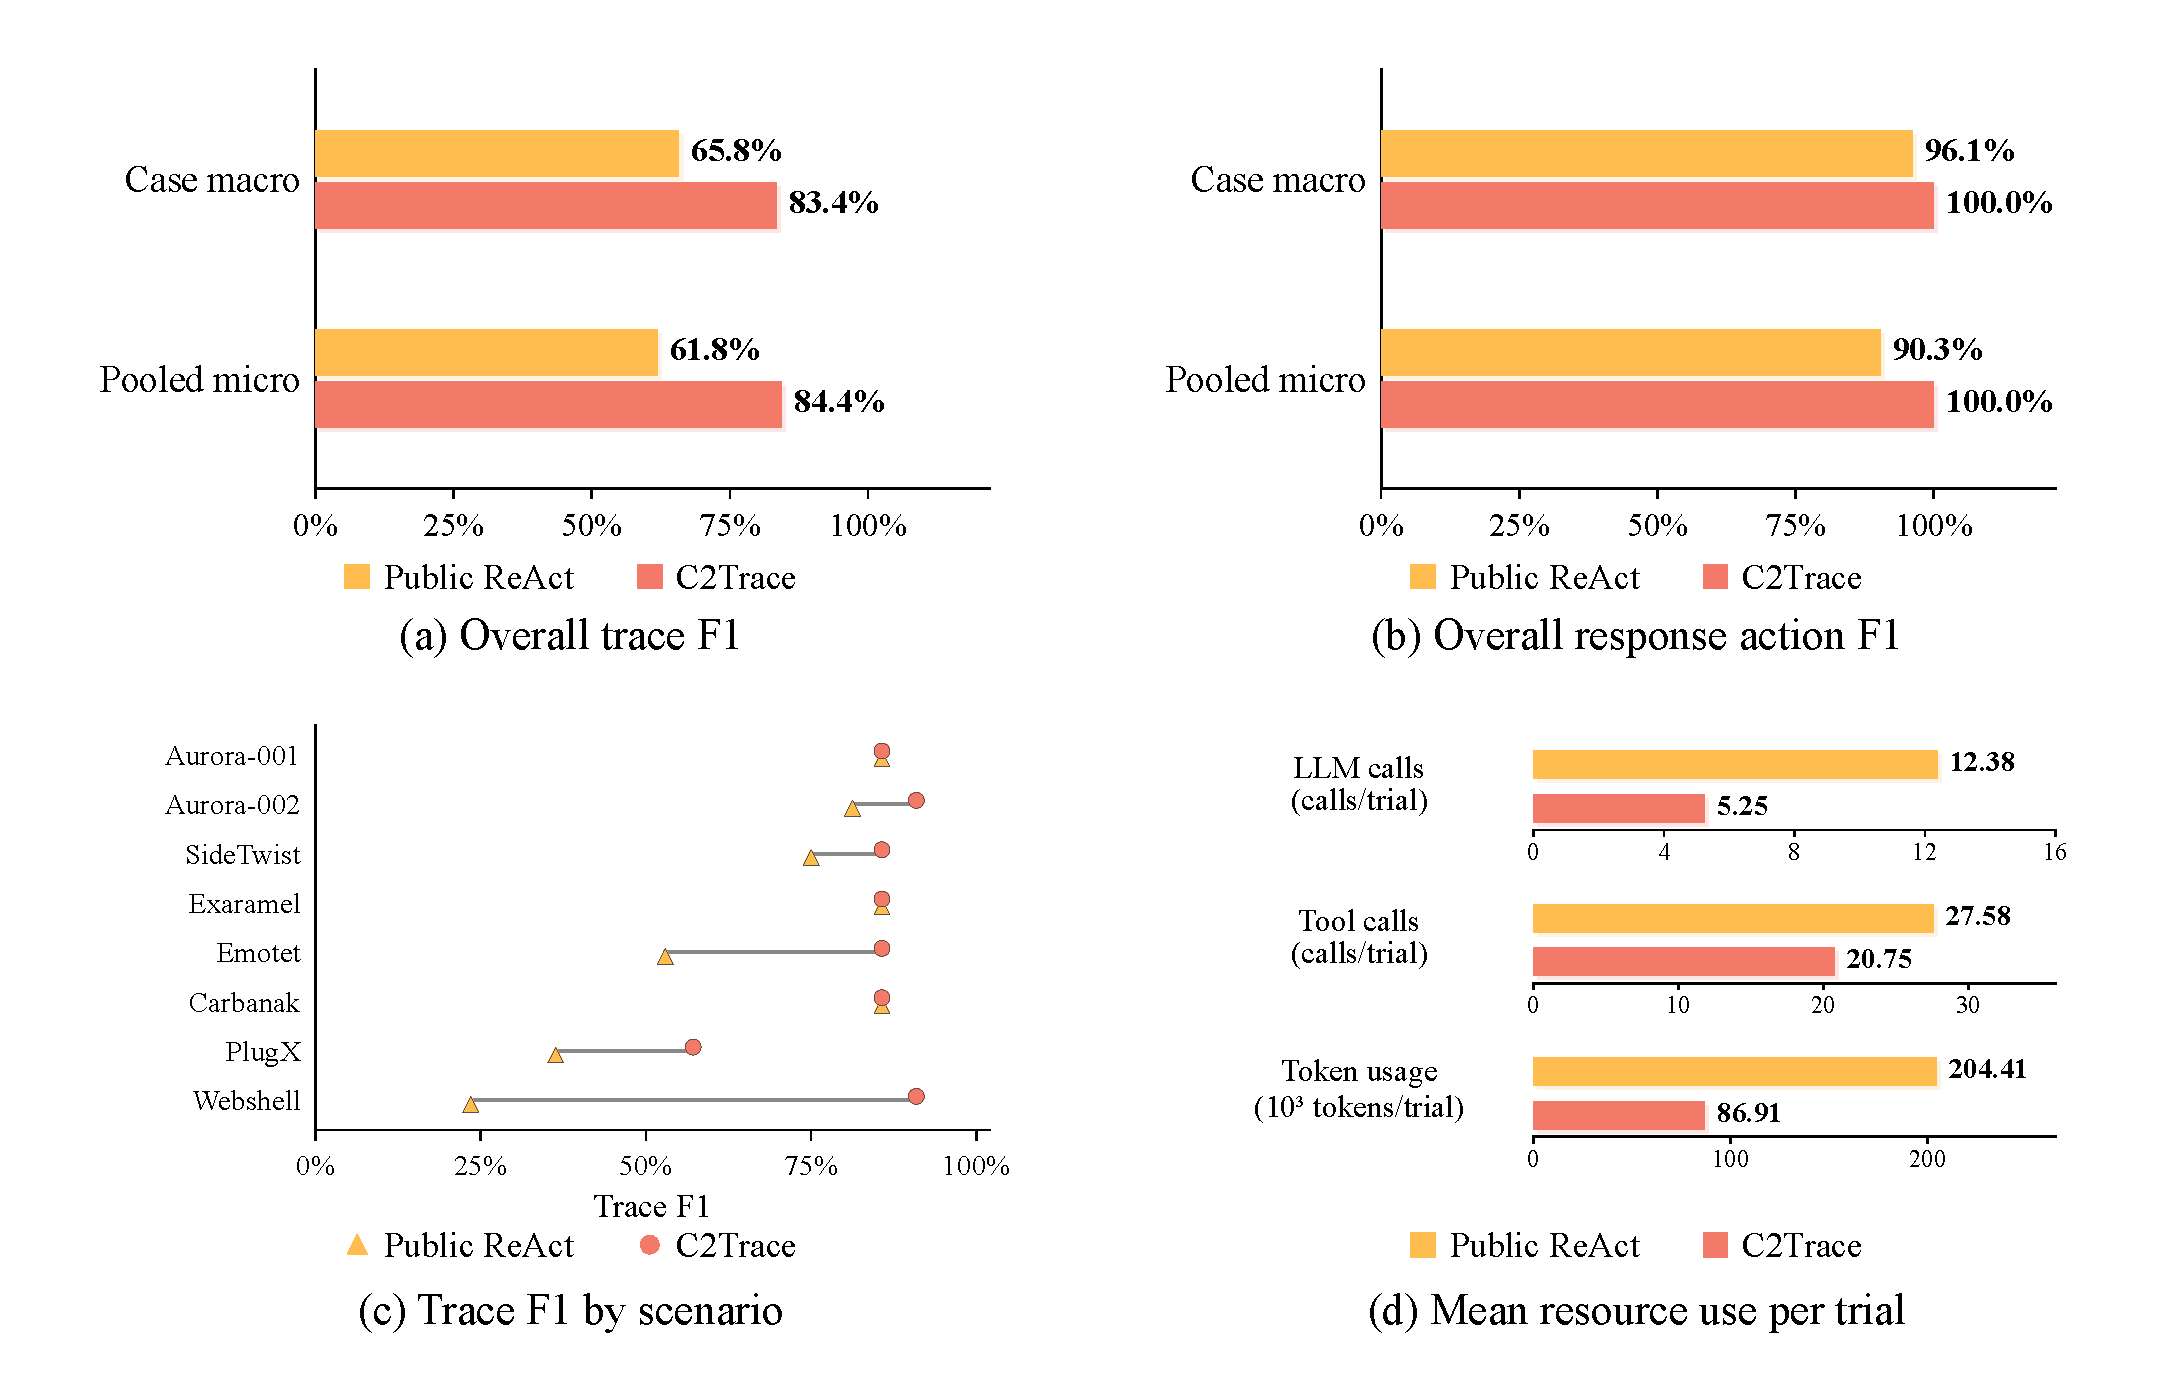
\includegraphics[width=\textwidth]{figures/rq2_comparison.pdf}
\caption{Effectiveness and resource usage of C2Trace and Public ReAct across eight scenarios, with three trials per system and scenario.}
\label{fig:rq2-comparison}
\end{figure}

\noindent\textbf{Investigation accuracy.} \system achieved a pooled trace F1 of 0.844, compared with 0.618 for Public ReAct. Its pooled precision and recall were 0.931 and 0.771, versus 0.591 and 0.648. Across the 105 reference facts in each system's 24 trials, \system recovered 81 and reported 6 unmatched observations, while Public ReAct recovered 68 and reported 47 unmatched observations. Thus, the higher F1 reflects both more recovered facts and fewer additional observations outside the reference. The macro F1 scores were 0.834 and 0.658, respectively (\autoref{fig:rq2-comparison}a). At the scenario level, \system had higher trace F1 in five cases and tied in Aurora 1, Exaramel, and Carbanak (\autoref{fig:rq2-comparison}c).

\noindent\textbf{Response effectiveness.} \system matched all 51 expected actions across its 24 trials, yielding pooled response precision, recall, and F1 of 1.000. Public ReAct matched 42 actions and missed 9, giving precision of 1.000, recall of 0.824, and F1 of 0.903. Its WebShell trials produced no response actions, leaving that scenario's precision and F1 undefined. Public ReAct's macro response F1 of 0.961 therefore averages seven defined scenarios, while \system's macro F1 of 1.000 covers all eight (\autoref{fig:rq2-comparison}b). Independent host checks passed in 24/24 trials for \system and 18/24 for Public ReAct. Overall trial classifications were 24 passes for \system and 12 passes for Public ReAct. Six additional Public ReAct trials passed the host checks but failed final-output validation because their observation schema rejected a \texttt{post\_state} field. This distinction accounts for the difference between its host-check results and overall pass count.

\noindent\textbf{Resource usage.} \system averaged 5.25 LLM calls, 20.75 tool calls, and 86,912.3 tokens per trial, compared with 12.38 calls, 27.58 tool calls, and 204,406.3 tokens for Public ReAct. Mean recorded token usage was 57.48\% lower for \system, with fewer LLM and tool calls across the evaluated trials (\autoref{fig:rq2-comparison}). The resource measures use separate zero-based axes, with calls reported per trial and token usage in thousands per trial. Mean end-to-end duration, including controller orchestration, was 159.4 seconds for \system and 142.5 seconds for Public ReAct, an increase of 11.85\%. The observed resource advantage therefore concerns model and tool usage, while completing \system's workflow took longer on average. These measurements cover each system's full trial under its configured workflow and resource limits.

We also compared \system with Offline Direct LLM to assess the findings and response proposals obtainable from a fixed evidence input. This baseline used \texttt{deepseek-v4.1-flash} at temperature 0.0 and performed one inference per scenario. Each inference received a frozen, de-labelled evidence bundle and produced structured findings and proposed actions. With zero host-tool calls, the baseline could interpret the supplied observations but could not query the host for additional evidence. We scored its reported facts and proposed operations and targets against the scenario references. \autoref{tab:direct} compares these scores with \system in the online RQ2 trials and reports mean token usage.

\noindent\textbf{Offline proposal quality.} Offline Direct LLM recovered 23 of 35 reference facts, missed 12, and reported 5 unmatched observations. Its micro trace F1 was 0.730 and macro F1 was 0.740. For action proposals, it matched 8 of 17 expected actions, missed 9, and proposed 11 unmatched actions, yielding micro and macro F1 scores of 0.444 and 0.458. For comparison, \system achieved micro F1 scores of 0.844 for trace facts and 1.000 for executed response actions in its online RQ2 trials. The offline scores reflect limited recovery of the reference facts and response targets from the fixed evidence input. The proposals were scored without host execution, and post-response host state was unmeasured. 

\begingroup
\let\table\tableorg
\let\endtable\endtableorg
\begin{table}[htbp]
\centering
\caption{Effectiveness and resource usage of \system and Public ReAct across eight Windows C2 scenarios, with three trials per system and scenario.}
\label{tab:baseline}
\small
\renewcommand{\arraystretch}{1.15}
\setlength{\tabcolsep}{3pt}
\resizebox{\linewidth}{!}{%
\begin{tabular}{lrrrrrr}
\toprule
\multicolumn{1}{l}{\multirow[c]{2}{*}[-0.5ex]{\textbf{System / task}}} & \multicolumn{3}{c}{\textbf{Case macro}} & \multicolumn{3}{c}{\textbf{Pooled micro}} \\
\cmidrule(lr){2-4}\cmidrule(lr){5-7}
 & \multicolumn{1}{c}{\textbf{P}} & \multicolumn{1}{c}{\textbf{R}} & \multicolumn{1}{c}{\textbf{F1}} & \multicolumn{1}{c}{\textbf{P}} & \multicolumn{1}{c}{\textbf{R}} & \multicolumn{1}{c}{\textbf{F1}} \\
\midrule
\rowcolor{black!6}
\system / Trace & 0.938 & 0.760 & 0.834 & 0.931 & 0.771 & 0.844 \\
\system / Response & 1.000 & 1.000 & 1.000 & 1.000 & 1.000 & 1.000 \\
\rowcolor{black!6}
Public ReAct / Trace & 0.698 & 0.655 & 0.658 & 0.591 & 0.648 & 0.618 \\
Public ReAct / Response & 1.000$^{7/8}$ & 0.812 & 0.961$^{7/8}$ & 1.000 & 0.824 & 0.903 \\
\midrule
\textbf{System} & \textbf{LLM calls} & \textbf{Tool calls} & \textbf{Tokens} & \textbf{E2E (s)} & \textbf{Pass} & \textbf{Fail} \\
\rowcolor{black!6}
\system & 5.25 & 20.75 & 86912.3 & 159.4 & 24 & 0 \\
Public ReAct & 12.38 & 27.58 & 204406.3 & 142.5 & 12 & 12 \\
\bottomrule
\end{tabular}%
}
\par\smallskip
\parbox{\linewidth}{\footnotesize
Each system has 24 trials. Superscripts indicate defined scenarios out of eight.
Usage and time are trial means. E2E includes controller orchestration.
Pass and Fail report overall trial classifications.}
\end{table}
\endgroup


% % Begin figures/figure05_baseline_f1.tex
% \begin{figure}[htbp]
% \centering
% 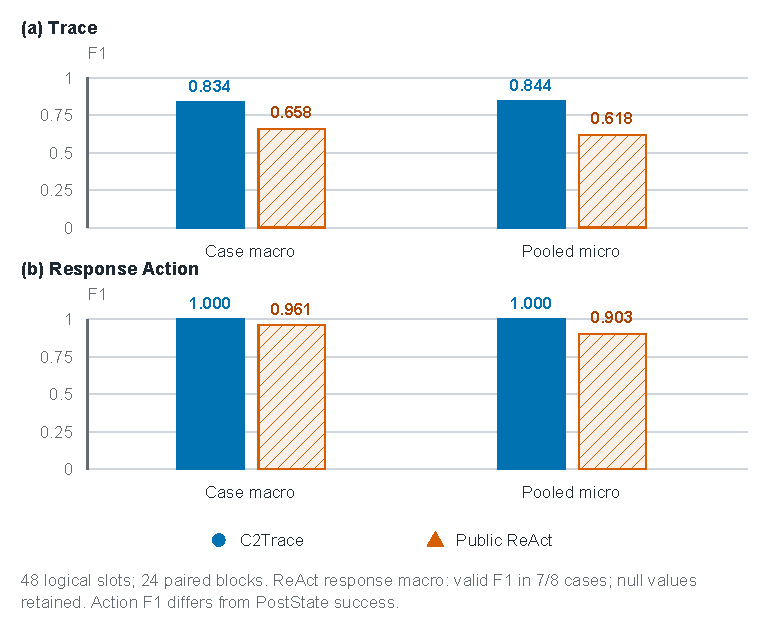
\includegraphics[width=\textwidth]{figures/figure05_baseline_f1.pdf}
% \caption{C2Trace and Public ReAct valid-trial baseline F1 over 48 logical slots and 24 paired blocks (8 cases, 3 repetitions per system). Case macro averages each case's aggregate metric; pooled micro combines all TP/FP/FN before computing F1. Public ReAct Response Action macro uses 7 of 8 cases because one case has no response predictions and its precision and F1 are reported as N/A under the scorer's convention. Action F1 is distinct from PostState success. LLM-Direct proposal metrics are excluded from this live comparison}
% \label{fig:baseline-f1}
% \end{figure}

% % End figures/figure05_baseline_f1.tex


% % Begin figures/figure06_case_trace_and_cost.tex
% \begin{figure}[htbp]
% \centering
% 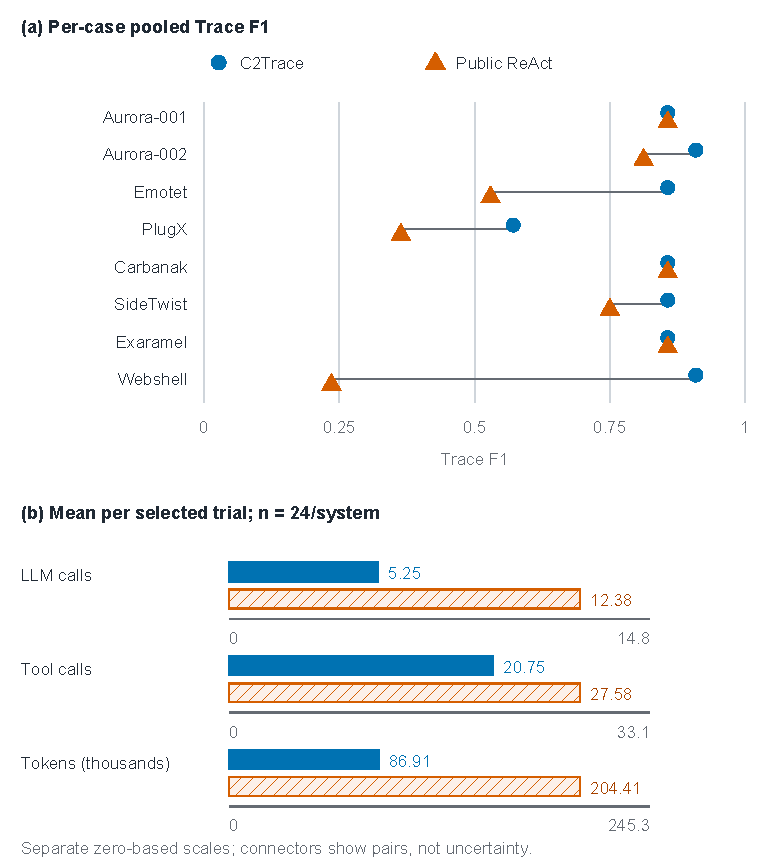
\includegraphics[width=\textwidth]{figures/figure06_case_trace_and_cost.pdf}
% \caption{Per-case pooled Trace F1 (upper panel) and mean LLM calls, tool calls and token usage per valid selected trial (lower panel) in the 48-slot live baseline. Each case has three trials per system; cost means have 24 selected trials per system, with valid field counts preserved in the source manifest. Cost panels use separate zero-based scales and different units, and token values are in thousands. Connecting lines show paired system values for each case, not uncertainty intervals. These observations are specific to the evaluated model and environment}
% \label{fig:case-cost}
% \end{figure}

% End figures/figure06_case_trace_and_cost.tex


\begingroup
\let\table\tableorg
\let\endtable\endtableorg
\begin{table}[htbp]
\centering
\caption{Effectiveness and resource usage of \system and Offline Direct LLM across eight Windows C2 scenarios.}
\label{tab:direct}
\small
\renewcommand{\arraystretch}{1.15}
\setlength{\tabcolsep}{3pt}
\begin{tabular}{lrrrr}
\toprule
\multicolumn{1}{l}{\multirow[c]{2}{*}[-0.5ex]{\textbf{Case}}} & \multicolumn{2}{c}{\textbf{Trace F1}} & \multicolumn{2}{c}{\textbf{Action F1}} \\
\cmidrule(lr){2-3}\cmidrule(lr){4-5}
 & \textbf{\system} & \textbf{Offline LLM}
& \textbf{\system} & \textbf{Offline LLM} \\
\midrule
\rowcolor{black!6}
C1: Aurora 1 & 0.857 & 0.857 & 1.000 & 0.500 \\
C2: Aurora 2 & 0.909 & 0.545 & 1.000 & 0.333 \\
\rowcolor{black!6}
C3: SideTwist & 0.857 & 0.571 & 1.000 & 0.500 \\
C4: Exaramel & 0.857 & 0.857 & 1.000 & 0.500 \\
\rowcolor{black!6}
C5: Emotet & 0.857 & 0.857 & 1.000 & 0.500 \\
C6: Carbanak & 0.857 & 0.857 & 1.000 & 0.500 \\
\rowcolor{black!6}
C7: PlugX & 0.571 & 0.571 & 1.000 & 0.500 \\
C8: WebShell & 0.909 & 0.800 & 1.000 & 0.333 \\
\midrule
\rowcolor{black!6}
Macro & 0.834 & 0.740 & 1.000 & 0.458 \\
Micro & 0.844 & 0.730 & 1.000 & 0.444 \\
\midrule
\textbf{Resource usage} & \multicolumn{2}{c}{\textbf{\system}}
& \multicolumn{2}{c}{\textbf{Offline LLM}} \\
Mean tokens per trial & \multicolumn{2}{c}{86,912.3}
& \multicolumn{2}{c}{3,213.8} \\
\bottomrule
\end{tabular}
\par\smallskip
\parbox{\linewidth}{\footnotesize
\system results use the 24 online RQ2 trials, with three runs per scenario.
Offline Direct LLM uses one inference per scenario.
Action F1 scores executed actions for \system and proposed actions for the offline baseline.}
\end{table}
\endgroup

\subsection{RQ3 (Component Analysis)}

We compared \system with three variants: A1 removes C2-KB and domain-specific guidance from the Planner's inputs; A2 disables automatic command-line payload-path extraction during investigation; and A3 removes the Auditor while retaining execution safeguards. Each configuration was evaluated three times on each of the eight scenarios, yielding 24 trials per configuration. A2 was collected subsequently using the same case definitions and scorer. \autoref{tab:ablation} reports investigation and response scores alongside resource usage, and \autoref{fig:ablation} shows the scores by scenario.

% Begin tables/table3_ablation.tex
\begingroup
\let\table\tableorg
\let\endtable\endtableorg
\begin{table}[!t]
\centering
\caption{Effectiveness and resource usage of \system and three ablation variants across eight Windows C2 scenarios, with three trials per configuration and scenario.}
\label{tab:ablation}
\small
\renewcommand{\arraystretch}{1.15}
\setlength{\tabcolsep}{3pt}
\renewcommand{\tabularxcolumn}[1]{m{#1}}
\newcommand{\ablationcell}[1]{\begin{tabular}[c]{@{}c@{}}#1\end{tabular}}
\resizebox{\linewidth}{!}{%
\begin{tabularx}{\linewidth}{l*{4}{>{\centering\arraybackslash}X}}
\toprule
\textbf{Case} & \begin{tabular}[c]{@{}c@{}}\textbf{C2Trace}\\Full system\end{tabular}
& \begin{tabular}[c]{@{}c@{}}\textbf{A1}\\No domain\\guidance\end{tabular}
& \begin{tabular}[c]{@{}c@{}}\textbf{A2}\\No command-line\\payload-path\\extraction\end{tabular}
& \begin{tabular}[c]{@{}c@{}}\textbf{A3}\\No Auditor\end{tabular} \\
\midrule
\rowcolor{black!6}
C1: Aurora 1 & \ablationcell{0.857\\1.000} & \ablationcell{0.133\\N/A} & \ablationcell{0.857\\1.000} & \ablationcell{0.857\\N/A} \\
C2: Aurora 2 & \ablationcell{0.909\\1.000} & \ablationcell{0.571\\0.500} & \ablationcell{0.714\\0.800} & \ablationcell{0.909\\N/A} \\
\rowcolor{black!6}
C3: SideTwist & \ablationcell{0.857\\1.000} & \ablationcell{0.500\\N/A} & \ablationcell{0.667\\0.800} & \ablationcell{0.857\\N/A} \\
C4: Exaramel & \ablationcell{0.857\\1.000} & \ablationcell{0.476\\N/A} & \ablationcell{0.667\\0.800} & \ablationcell{0.857\\N/A} \\
\rowcolor{black!6}
C5: Emotet & \ablationcell{0.857\\1.000} & \ablationcell{N/A\\N/A} & \ablationcell{0.444\\0.500} & \ablationcell{0.857\\N/A} \\
C6: Carbanak & \ablationcell{0.857\\1.000} & \ablationcell{0.471\\N/A} & \ablationcell{0.571\\0.667} & \ablationcell{0.857\\N/A} \\
\rowcolor{black!6}
C7: PlugX & \ablationcell{0.857\\1.000} & \ablationcell{0.250\\N/A} & \ablationcell{0.571\\N/A} & \ablationcell{0.857\\N/A} \\
C8: WebShell & \ablationcell{0.909\\1.000} & \ablationcell{0.300\\N/A} & \ablationcell{0.909\\1.000} & \ablationcell{0.909\\N/A} \\
\midrule
\rowcolor{black!6}
Macro F1 & \ablationcell{0.870\\1.000} & \ablationcell{0.386$^{7/8}$\\0.500$^{1/8}$} & \ablationcell{0.675\\0.795$^{7/8}$} & \ablationcell{0.870\\N/A$^{0/8}$} \\
Micro F1 & \ablationcell{0.875\\1.000} & \ablationcell{0.379\\0.111} & \ablationcell{0.697\\0.756} & \ablationcell{0.875\\N/A} \\
\rowcolor{black!6}
Response recall & 1.000 & 0.059 & 0.608 & 0.000 \\
PostState passed & 24/24 & 1/24 & 12/24 & 0/24 \\
\rowcolor{black!6}
Tool calls (sum) & 492 & 76 & 373 & 246 \\
LLM calls (sum) & 126 & 30 & 89 & 24 \\
\rowcolor{black!6}
Tokens (sum) & 1,980,355 & 220,736 & 1,234,470 & 166,729 \\
Tokens (mean) & 82,514.8 & 9,197.3 & 51,436.3 & 6,947.0 \\
\bottomrule
\end{tabularx}%
}
\par\smallskip
\parbox{\linewidth}{\footnotesize
Case and aggregate F1 cells show trace above response F1.
Each configuration includes three trials per scenario; counts are pooled within each scenario before computing case scores and macro averages.
N/A follows the scorer's convention for empty prediction sets. Macro superscripts give the number of defined cases when fewer than eight. Response recall is micro-averaged over all trials.
PostState is measured before external cleanup.
Resource sums and means cover 24 trials per configuration.
A2 includes first-request transport failures in the third repetition of C2--C5; their token usage was not returned.}
\end{table}
\endgroup


\begin{figure}[!t]
\centering
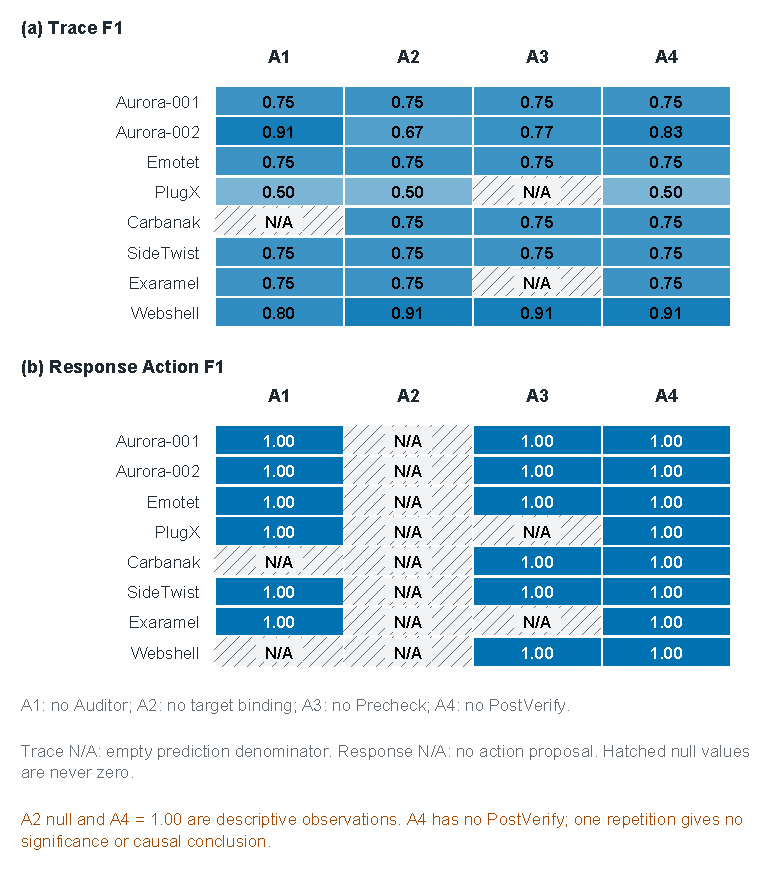
\includegraphics[width=0.92\textwidth]{figures/figure07_ablation_heatmap.pdf}
\caption{Trace and response action F1 of \system and three ablation variants across eight Windows C2 scenarios, with three trials per configuration and scenario.}
\label{fig:ablation}
\end{figure}

\noindent\textbf{Domain-guided planning.} A1 retained the same Planner model, supplied with the alert, tool descriptions, and required output format. Its pooled trace F1 decreased from 0.875 to 0.379 and response F1 from 1.000 to 0.111. It recovered 29 of 105 reference facts and completed 3 of 51 expected response actions; only one trial passed the independent host checks. Ten trials stopped during planning after selecting a tool reserved for controller-managed investigation. The reduction includes both incomplete evidence recovery and rejection of plans that violated tool-selection constraints. It therefore reflects the combined removal of C2 knowledge and planning guidance.

\noindent\textbf{Command-line payload extraction.} A2 achieved pooled trace and response F1 of 0.697 and 0.756, respectively, with 12 of 24 trials passing the host checks. Four trials failed at the first model request because of transport errors and remain in these totals. Excluding the C5 transport failure, none of the eight remaining trials across C5--C7 removed the target payload file, whereas \system did so in all eight corresponding trials. In C5 and C6, the target processes were stopped, but file candidates referred to the system host programs and were rejected by the Auditor's protection rules, leaving the loaded DLL or script intact. In C7, the candidate file differed from the locked target, preventing execution. These outcomes distinguish identifying a connection-owning process from locating the separate payload that must be removed.

\noindent\textbf{Independent auditing.} A3 retained the full system's pooled trace F1 of 0.875 but completed none of the 51 expected response actions. Response recall was zero, with precision and F1 reported as N/A. In all 24 trials, a registry-removal candidate without a matching locked target reached the downstream safety check and prevented execution. Thus, unchanged investigation accuracy did not ensure that the response plan could proceed. Auditing affected the selection of supported response candidates before execution; with that step removed, the remaining safeguards rejected the plans. No unsupported action was actually executed in these trials.

\noindent\textbf{Resource usage.} Mean recorded token usage was 82,514.8 for \system, compared with 9,197.3, 51,436.3, and 6,947.0 for A1--A3. All 24 full-system trials entered response execution, compared with one for A1, 17 for A2, and none for A3. The lower costs therefore include early termination and omitted response execution, and do not indicate equivalent task completion at lower cost.

\section{Discussion}
\label{sec:discussion}

\subsection{Implications}

\noindent\textbf{Action-Specific Evidence.} The results suggest organizing automated response around the evidence required for each operation. Partial investigation can support a correct response, while identifying a connection-owning process can still leave its payload unresolved. A process instance, its executable, and its loaded payload therefore need distinct identities and evidence links. This distinction allows the workflow to assess termination and file removal separately, connecting investigation findings to explicit conditions for modifying software objects.

\noindent\textbf{Screening and Execution Control.} Candidate screening and execution checks serve complementary purposes. The auditing analysis shows that downstream safeguards can reject an unsupported proposal while leaving the response incomplete. Screening determines which evidence-supported candidates advance, whereas execution checks revalidate the prepared operation against the current target. For automated workflows, this separation motivates assessing both rejection behavior and task completion: preventing an inadmissible operation and completing an admissible one are distinct outcomes.

\noindent\textbf{Verification of Observable Effects.} Automated response should be evaluated through observed host changes alongside action records and report validity. The baseline comparison showed that completed host changes could coexist with an invalid final report. Fresh PostState checks make these outcomes distinguishable and connect evaluation to the intended operational effect. Completion also provides context for efficiency measurements, since early termination reduces resource use and fewer model calls do not necessarily produce lower end-to-end latency.

\subsection{Limitations}

The findings concern eight controlled Windows scenarios and one LLM, limiting generalization across models, platforms, and incident complexity. Workflow differences, combined component removals, and transport failures restrict attribution of the observed gains to individual mechanisms. The live comparison measures selected service-valid executions rather than first-attempt availability. Trace scores measure agreement with registered facts, and undefined F1 values give macro averages different scenario coverage. Independent host checks cover specified targets and controls rather than complete incident eradication. Authorization and target revalidation remain non-atomic, with in-memory replay protection and weaker checks for sibling termination. The historical protected-object incident and the absence of adversarial injection or exhaustive race testing further limit safety conclusions.  

\section{Related Work}
\label{sec:related}

\subsection{Provenance and Attack Investigation}

Provenance-based investigation represents relationships among processes, files, and communications to recover attack activity. Dependency reconstruction and selective collection support tracing intrusion origins while managing logging overhead and dependency growth~\citep{backtracker2003,protracer2016}. Audit records and information flows further enable attack-scenario reconstruction, correlation across attack stages, and provenance-based detection and investigation~\citep{sleuth2017,holmes2019,kairos2024}. These methods provide a basis for understanding how an intrusion unfolded. Reconstructed relationships alone, however, do not establish whether a particular operation remains applicable to a current host object. \system addresses this transition by linking observations to operation-specific targets and revalidating their identities before execution.

\subsection{Playbooks and Automated Response}

Automated response research addresses workflow representation, action selection, and operational constraints. CACAO specifies exchangeable workflows, conditions, commands, and targets, while OpenC2 provides an interoperable action--target command language~\citep{cacao2023,openc2-2019}. Response-selection methods incorporate attack-graph dependencies~\citep{adepts2005}, game-theoretic models of response and recovery~\citep{rre2014}, and estimates of response costs based on resource and operational dependencies~\citep{orcef2015}. These contributions support expressing and choosing responses, while the evidence needed to authorize a concrete host operation and verify its effect remains a separate concern. \system focuses on this execution boundary through evidence checks, argument-bound authorization, and fresh observations of the affected host objects.

\subsection{LLM Assistance in Incident Response}

LLM assistance in incident response supports context-dependent recommendations and the integration of generated information into analysts' work. Guided Response uses incident context to recommend investigation, triage, and remediation steps~\citep{guided-response2025}, while studies of analyst workflows examine the role of LLM assistance and identify limitations of autonomous summarization~\citep{kramer2025}. Together, these works inform how model outputs can support incident interpretation and response decisions. Recommendations and summaries alone do not establish the evidence or execution conditions required to modify a specific host object. \system connects generated strategies to host actions through structured dependencies, evidence-resolved targets, and deterministic audit and execution checks.

\section{Conclusion}
\label{sec:conclusion}

In this paper, we presented \system, an automated workflow that connects C2 alerts to evidence-supported investigation and verified response on Windows hosts. The system combines knowledge-guided planning and shared case memory with action-specific auditing, target-bound authorization, and fresh host verification. Its core contribution is to link generated strategies to explicit conditions for modifying host objects and to observed execution outcomes. Across eight controlled scenarios, the live comparison with Public ReAct yielded pooled trace F1 of 0.844 versus 0.618 and response action F1 of 1.000 versus 0.903. Independent host checks passed in 24/24 trials for \system and 18/24 for Public ReAct. \system also used fewer model and tool calls, with lower token usage but higher end-to-end latency. These findings support the use of explicit evidence links, execution conditions, and outcome checks in engineering automated investigation and response workflows.

\backmatter
\section*{Statements and Declarations}

\noindent\textbf{Funding.}
This work was partly supported by the National Natural Science Foundation of China (grant Nos. 62672193 and 62572209) and the Hubei Provincial Key Research and Development Program (grant No. 2025BAB057).

\medskip
\noindent\textbf{Competing interests.}
The authors declare no competing interests.

\medskip
\noindent\textbf{Author contributions.}
The authors contributed to the study design, system development, experimental evaluation, and manuscript preparation. All authors reviewed and approved the final manuscript.

\medskip
\noindent\textbf{Data and code availability.}
The source code, scenario definitions, and experimental data supporting this study are available from the corresponding author upon reasonable request.

\medskip
\noindent\textbf{AI assistance.}
The authors directed the research and determined the manuscript's scientific arguments, interpretation of results, and conclusions. OpenAI Codex was used to assist with manuscript preparation. The authors checked the text against the study methods and experimental evidence, revised its wording and organization, and take full responsibility for the accuracy and integrity of the final manuscript.

\appendix
\section{Artifact, Trial Selection, and Audit Boundaries}
\label{sec:artifact}

\subsection{Evidence Organization}

The supporting records are organized by research question, scenario, and trial. For RQ1, the retained materials include scenario references, CaseFiles, investigation and response scores, resource measurements, and independent post-response host checks. The live RQ2 comparison retains scores, trial classifications, resource measurements, and host checks for 48 selected valid trials. For the Offline Direct LLM baseline in RQ2, the records contain fixed evidence inputs, model outputs, and scores for reported facts and proposed actions from eight inferences, with no host execution or post-response host measurements. RQ3 records cover the 96 trials in \autoref{tab:ablation} and include scores, trial outcomes, resource measurements, CaseFiles, independent host checks, and environment-recovery records.

Source manifests identify the records and aggregation formulas underlying the reported results, with SHA-256 hashes supporting file-integrity checks. The original experimental records are preserved unchanged. For the live RQ2 comparison, we checked stored scores against their matching records and recomputed count-based metrics, macro averages across scenarios, and pooled micro metrics. These checks assess consistency among retained scoring outputs and aggregates; they do not constitute an independent rerun of the original scorer.

\subsection{Case Keys and Source Fidelity}

Tables and figures use the following case keys consistently:
\begin{center}
\begin{tabular}{@{}ll@{}}
C1 & \texttt{AURORA-CHAIN-001} \\
C2 & \texttt{AURORA-CHAIN-002} \\
C3 & \texttt{AEL-OILRIG-SIDETWIST-001} \\
C4 & \texttt{AEL-SANDWORM-EXARAMEL-WIN-001} \\
C5 & \texttt{AEL-WIZARD-EMOTET-001} \\
C6 & \texttt{AEL-CARBANAK-RAT-001} \\
C7 & \texttt{AEL-MUSTANG-PANDA-PLUGX-001} \\
C8 & \texttt{MEP-WINDOWS-WEBSHELL-01}
\end{tabular}
\end{center}
Full IDs and source commits are retained in the companion rather than using family names as fidelity certificates. Reproducing a selected C2 channel or host artifact is narrower than reproducing an entire upstream campaign. Measured transport, scenario semantics, actual carrier, and scoring facts are separate fields.

\subsection{Selected Slots and Preserved Earlier Events}

\autoref{fig:provenance} maps eligibility and logical slots to selected runs, original score and PostState artifacts, offline arithmetic checks, and reproducible aggregates. Each system contributes three valid selected runs per case. A selected run occupies an existing slot and does not create an additional observation; the companion retains the exact slot-to-run mapping and source hashes. Selection uses the symmetric service-availability and setup-validity criterion described in RQ2 and retains normal-output evaluation failures. The historical protected-object safety incident remains separate from ordinary performance scoring.

The resulting population measures complete-system behavior in valid executions rather than an unmodified first-attempt availability sequence. Recorded cleanup success, trial classification, scored action matches, and independent fresh PostState have distinct denominators and meanings. Paired comparisons retain undefined metrics and never translate an undefined difference into a win or loss.

% Begin figures/figure08_provenance.tex
\begin{figure}[htbp]
\centering
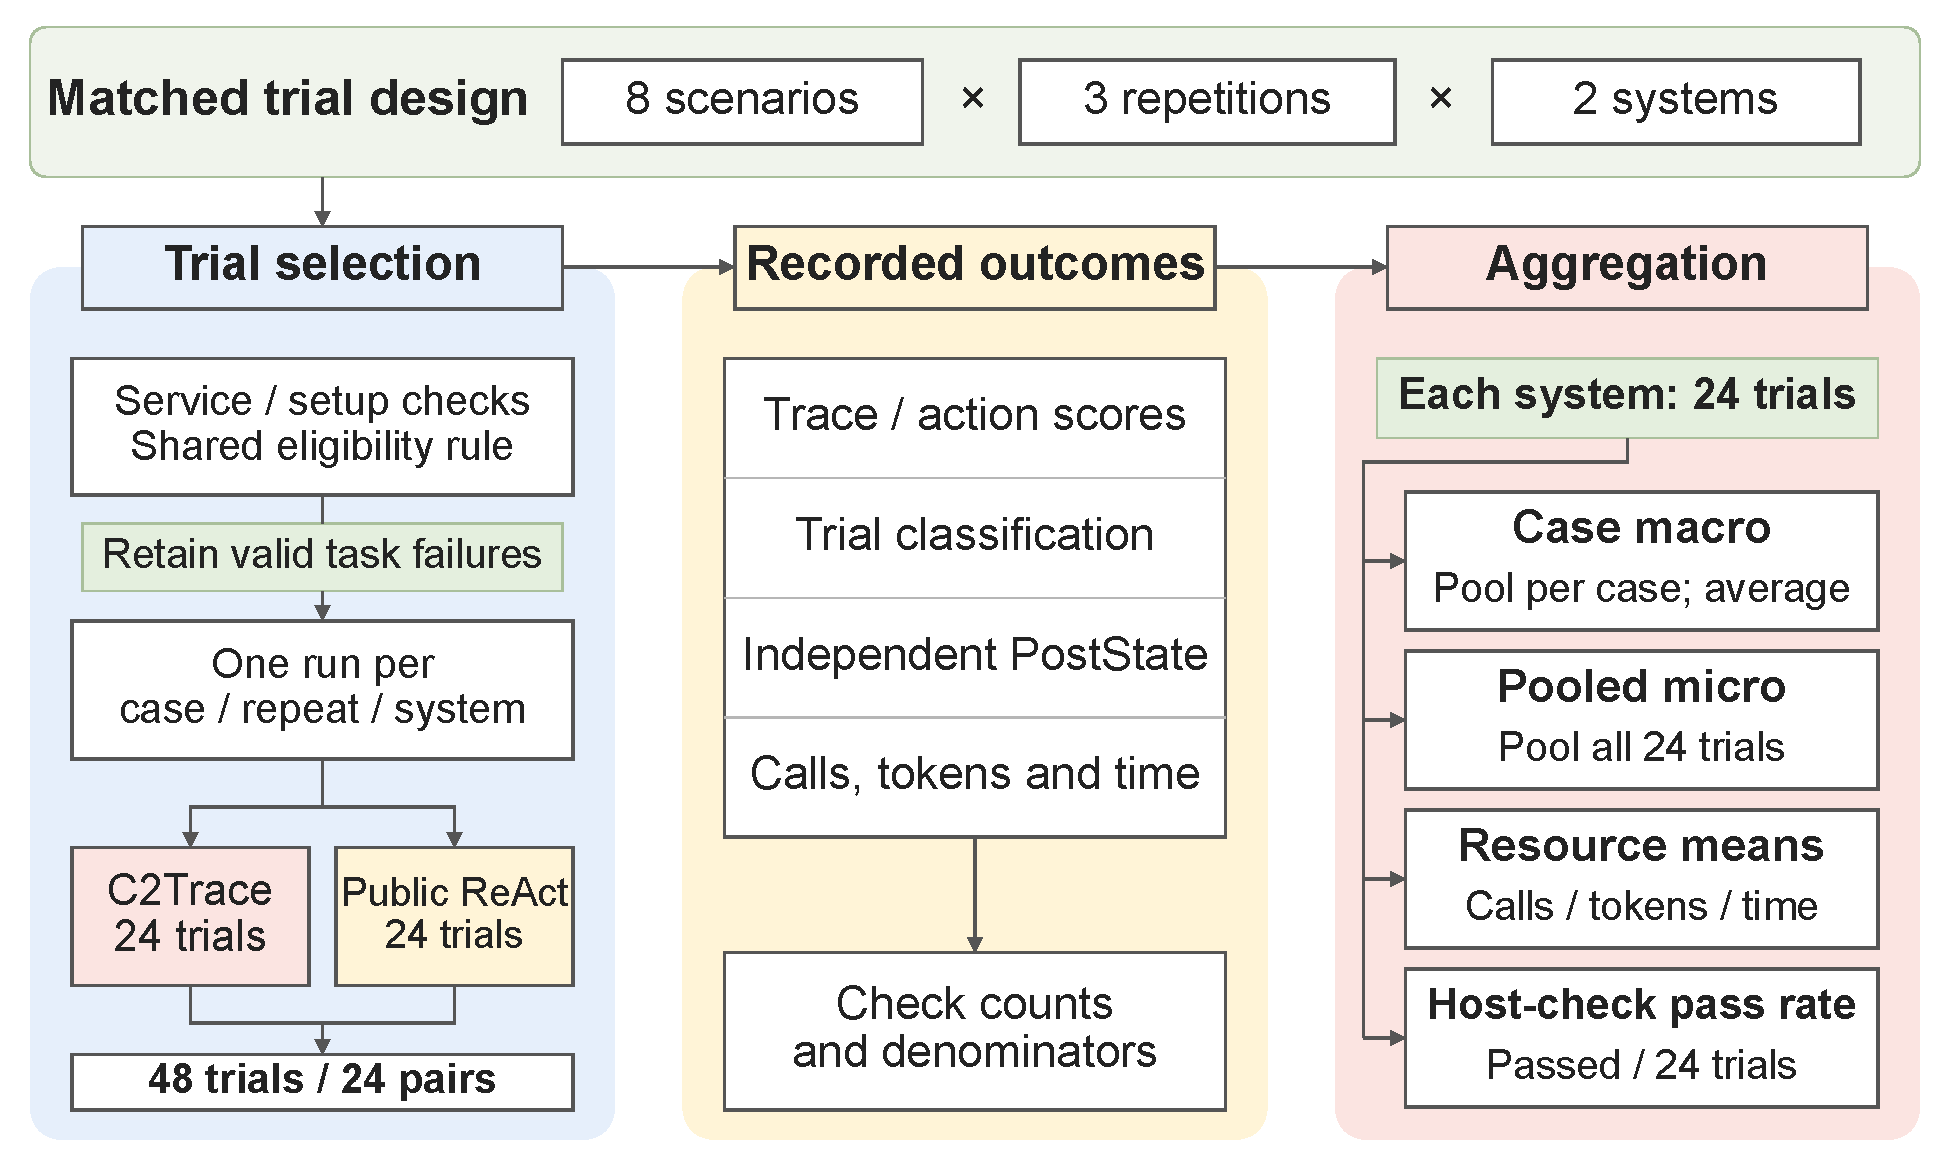
\includegraphics[width=\textwidth]{figures/figure08_provenance.pdf}
\caption{Overview of trial selection and result aggregation for the live comparison. Shared service and setup checks select 24 trials per system across eight scenarios, retaining valid task failures and forming 24 matched pairs. The retained records link investigation and response scores, trial classifications, independent host checks, and resource measurements to the reported macro and micro scores, resource means, and host-check pass rates.}
\label{fig:provenance}
\end{figure}

% End figures/figure08_provenance.tex


\subsection{Experimental Records}

\autoref{tab:boundaries} summarizes the trial populations and retained records supporting verification of the reported results.

% Begin tables/table6_boundaries.tex
\begin{table}[htbp]
\centering
\caption{Overview of trial counts and retained experimental records across the evaluation groups.}
\label{tab:boundaries}
\small
\setlength{\tabcolsep}{4pt}
\begin{tabularx}{\textwidth}{@{}p{32mm}p{19mm}X@{}}
\toprule
Evaluation & Trials & Retained records \\
\midrule
RQ1: Effectiveness & 8 &
Scores, resource usage, and independent host checks \\
RQ2: Live comparison & 48 &
Scores, trial classifications, resource usage, and independent host checks \\
RQ2: Offline Direct LLM & 8 &
Fixed evidence inputs, model outputs, and action-proposal scores \\
RQ3: Component analysis & 96 &
Scores, trial outcomes, resource usage, independent host checks, and environment-recovery records \\
\bottomrule
\end{tabularx}
\end{table}
% End tables/table6_boundaries.tex


\subsection{Implementation Version and Context Projection}

The experimental findings apply to the implementations and configurations used in the evaluated trials. The reported investigation and action scores and resource measurements are derived from the retained trial records. For the live experiments, response outcomes are additionally assessed through independent host checks performed before environment recovery. These records provide the basis for verifying the reported results and interpreting the observed system behavior.

The compact CaseFile view excludes dedicated top-level safety fields while retaining prior audit/action receipts, which can contain evidence-derived authorization claims. It is therefore a restricted projection, not a guarantee that all identity information is recursively removed. Ground Truth separation is supported by the inspected entrypoint and available input-boundary evidence.

% \subsection{Artifact Reconstruction}

% The companion includes the evidence map, source manifest, verified result JSON, displayed-table bindings, figure source records, and generation scripts. Rebuilding tables and figures reads these files only. Original experiment artifacts, scorer, protocols, and schedules are unmodified. Numerical figures are vector PDFs with values sourced from the same verified data; the architecture figure is retained as a raster image.

% The valid-trial comparison includes separately collected completion runs. Reconstruction of the tables and figures is performed offline using retained experimental records, without invoking model APIs, conducting live experiments, or rerunning the original scorer.

\clearpage
\bibliography{references}
\end{document}
